% File:		vec-2d.tex
% Author:	See Below
% Date:	        See Below
%
% The authors have placed this file in the public domain;
% they make no warranty and accept no liability for this file.

\documentclass[12pt]{article}
\usepackage{times}
\usepackage{color}
\usepackage[usenames]{xcolor}
\usepackage{scalefnt}
\usepackage{tikz}
\usepackage{wrapfig}
\usetikzlibrary{arrows}
\begin{document}
\newcommand{\header}[1]{\underline{\bf #1}}
\newcommand{\file}[1]{{\bf #1}}
\newcommand{\blankpage}{\newpage\vspace*{3.5in}%
    \centerline{\Large This Page is Intentionally Left Blank}}
\setlength{\parindent}{0.0in}
\setlength{\parskip}{1ex}
\newcommand{\key}[1]{{\bf #1}}
\newcommand{\TT}[1]{{\tt \bfseries #1}}
\newcommand{\EOL}{\penalty \exhyphenpenalty}
\newtheorem{definition}{Definition}[section]
\newtheorem{lemma}[definition]{Lemma}
\newtheorem{corollary}[definition]{Corollary}
\newtheorem{theorem}[definition]{Theorem}
\newenvironment{indpar}[1]%
    {\begin{list}{}{\setlength{\leftmargin}{#1}}\item[]}%
    {\end{list}}

\section{Two Dimensional Geometry Calculator}
This document describes a group of 2-dimensional geometry problems,
starting with simple vector calculations, and working up to polygons and
ellipses.
The problems are embedded in a simple calculator for ease of
testing.

\section{Boolean, Scalars, Vectors, and Transforms}
A \key{boolean} here is either the symbol \key{true} or the symbol \key{false}.

A \key{scalar} here is a double precision floating point number.

A \key{vector} here is a pair $(x,y)$ of double precision floating point
numbers, $x$ denoting an X-coordinate value, and $y$ denoting a
Y-coordinate value.  Such a vector can denote a point $(p_x,p_y)$ in the
XY-plane, or can denote a translation $(v_x,v_y)$ of the plane: \\
\centerline{$(p_x,p_y) \longmapsto (p_x+v_x,p_y+v_y)$}

The product of a scalar $s$ and a vector $v=(v_x,v_y)$ is represented using
$*$ as $s*v = (sv_x,sv_y)$.
The sum of a vector $v=(v_x,v_y)$ and a vector $w=(w_x,w_y)$ is
represented using $+$ as $v+w = (v_x+w_x,v_y+w_y)$.

A \key{linear transformation} here is a pair of vectors, $[\ell_x,\ell_y]$
representing the map:
\centerline{$(v_x,v_y) \longmapsto v_x*\ell_x+v_y*\ell_y$}
Application is represented using
$*$ as $[\ell_x,\ell_y]*v=v_x*\ell_x+v_y*\ell_y$.

A \key{vector list} here is a list of vectors
$(v_1,v_2,\ldots)$.  This can be used to represent the list of vertices
of a polygon or a list of points in the plot of a function.

\newpage

\section{The Calculator Language}
The calculator language of this problem is very simple.
An example is:
\\[1ex]
{\tt
\hspace*{0.2in}\begin{tabular}{l@{\hspace{0.5in}}l}
\rm \bf Input	& \rm \bf Output \\\hline
x=4		& x=4 \\
y = 0.5         & y = 0.5 \\
z = x + y       & z = x + y = 4.5 \\
v=(3,-2)	& v=(3,-2) \\
w=z*v		& w=z*v = (13.5,-9) \\
\# this is a comment & \# this is a comment
\end{tabular}
} % \tt

The syntax is:
\\[1ex]
\hspace*{0.2in}\begin{tabular}{l}
{\em program} ::= {\em statement}$^\star$ \\
{\em statement} ::= \\
\hspace*{0.2in}\begin{tabular}[t]{cl}
                    & {\em comment} {\em eol} \\
                $|$ & {\em variable} \TT{=} {\em value} {\em eol}\\
                $|$ & {\em variable} \TT{=} {\em operator}
		          \{ {\em variable} {\em operator} \}$^\star$
		          {\em variable}$^?$ {\em eol} \\
                $|$ & {\em variable} \TT{=} {\em variable}
		          \{ {\em operator} {\em variable} \}$^\star$
		          {\em operator}$^?$ {\em eol} \\
                $|$ & {\em variable} \TT{=} {\em function}
		          {\em variable}$^\star$ {\em eol} \\
		\end{tabular}
\\[1ex]
{\em eol} ::= end-of-line (line-feed) \\
{\em comment} ::= \TT{\#} {\em character-other-than-line-feed}$^\star$ \\
{\em variable} ::= a single letter (case matters) \\
{\em value} ::= {\em boolean} $|$ {\em scalar} $|$ {\em vector}
	    $|$ {\em linear-transform} $|$ {\em vector-list} \\
{\em boolean} ::= \TT{true} $|$ \TT{false} \\
{\em scalar} ::= \begin{tabular}[t]{@{}l}
                 double precision floating point number (e.g., 1.4142135) \\
		 (must have a digit before any decimal point) \\
		 \end{tabular} \\
{\em vector} ::= \TT{(} {\em scalar}\TT{,} {\em scalar} \TT{)} \\
{\em linear-transform} ::= \TT{[} {\em vector}\TT{,} {\em vector} \TT{]} \\
{\em vector-list} ::= \TT{()} $|$
                 \TT{(} {\em vector} \{ \TT{,} {\em vector} \}$^\star$ \TT{)} \\
{\em operator} ::= \begin{tabular}[t]{@{}l}
                   one or more non-letter, non-digit graphic characters \\
                   (e.g. {\tt +} or {\tt <=})\\
		   \end{tabular} \\
{\em function} ::= three or more letters (e.g. {\tt sin} or {\tt area})
\end{tabular}

The Input/Output Rules are:
\begin{indpar}{0.2in}\begin{itemize}

\item Whitespace in {\em statements} is optional and should be deleted
before the {\em statements} are parsed.  There may be whitespace
before the `{\tt \#}' that begins a comment.

\item The output of a {\em statement} is a copy of the {\em statement},
which if the {\em statement} is neither a comment nor of the form
`{\em variable} \TT{=} {\em value} {\em eol}', 
is followed by `{\em space} \TT{=} {\em space} {\em value}', where
the {\em value} is that assigned to the {\em variable} beginning the
statement.

\item Input lines have a maximum of 100,000 characters (long lines
are only needed for inputting vector lists).  Output lines have
no limit (output vector lists can be arbitrarily long).

\item Each calculator version should be able to input and output
values of the types being tested by that version (beginning with
{\em boolean} and {\em scalar} values) and process comments
and statements of the form `{\em variable} \TT{=} {\em variable}'.

\item {\em Scalars} should be output with 6 digits of precision
(which is the default for C/C++).  To pass tests, scalar values
must be accurate to better than 5 digits of precision \underline{or}
to better than $\pm 10^{-6}$.

\item  The total number of vector list elements that need to be
allocated during one program execution will be small enough
that these list elements do not need to be garbage collected
(need not be freed when no longer needed).

\item Input will \underline{not} contain the character `{\tt \$}',
which can then be used as per Coding Hints below.


\end{itemize}\end{indpar}

\newpage

\section{Scalar Calculator}
Implement the calculator with just {\em scalar} and {\em boolean}
value types and the 
{\em operators} and {\em functions}:
\begin{center}
\begin{tabular}{l@{~~~~~}l}
Assume:	& {\tt x=}$x$, {\tt y=}$y$ (scalars) \\
	& {\tt d=}$d$ (an integer scalar $0\le d\le 12$) \\
	& {\tt b=}$b$ (a boolean) \\
then: \\[1ex]
\tt x+y & returns $x + y$ \\
\tt x-y & returns $x - y$ \\
\tt x*y & returns $x \times y$ \\
\tt x/y & returns $x / y$ \\
\tt x\%y & returns remainder of $x/y$ rounded to integer nearest zero \\
\tt -x & returns $-x$ \\
\tt |x| & returns $|x|$, the absolute value of $x$ \\
\tt cos x & returns $\cos ( (\pi/180) * x )$ [{\tt x} is in degrees] \\
\tt sin x & returns $\sin ( (\pi/180) * x )$ [{\tt x} is in degrees] \\
\tt tan x & returns $\tan ( (\pi/180) * x )$ [{\tt x} is in degrees] \\
\tt x<y:d & returns \TT{true} if $x<y-0.5*10^{-d}$, else \TT{false} \\
\tt x<=y:d & returns \TT{true} if $x<y+0.5*10^{-d}$, else \TT{false} \\
\tt x==y:d & returns \TT{true} if $|x-y|<0.5*10^{-d}$, else \TT{false} \\
\end{tabular}
\end{center}

Angles are measured in degrees, with positive angles going counter-clockwise
and negative angles going clockwise.

Comparisons assume the scalars being compared are approximations
to precise numbers that are in units of $10^{-d}$, and therefore to test
for equality the scalars should be (in effect) rounded to the nearest unit.
In addition, the scalars have to be good enough approximations.  As
\label{DOUBLE-SIZE-LIMITS}
double precision floating point numbers are accurate to at most one part
in $10^{16}$, this means that if the units are $10^{-d}$ the scalar
should not have absolute value above $10^{15-d}$.

Division by {\tt 0} will produce results such as
{\tt inf} (plus infinity), {\tt -inf} (minus infinity),
and {\tt nan} (not a number; i.e., result could not be computed).

\begin{center}
\begin{tabular}{rl}
Sample Input Files: & \file{00-XXXX-scalar-vec-2d.in} \\
Sample Output Files: & \file{00-XXXX-scalar-vec-2d.ftest} \\
Sample Run File: & \file{sample-scalar-vec-2d.run} \\
Submit Run File: & \file{submit-scalar-vec-2d.run} \\
\end{tabular}
\end{center}

You can test your program using the indicated sample input and
output and you can submit your program using the indicated submit
run file.  Only scalar functionality is tested.

There is also an input file:
\begin{center}
\begin{tabular}{rl}
Sample Input Files: & \file{00-000-special-vec-2d.in} \\
\end{tabular}
\end{center}
which may be used to test the results of divide by zero
and other anomolous scalar computations.
The output of your program for this file will depend
upon the programming language you use, so the output is
not testable except by human inspection.  Therefore this {\tt .in}
file is not included in any {\tt .run} files.

\section{Coding Hints}
The calculator memory just maps each variable to a value.
You can map each ASCII character to a value using a
vector of 128 elements, and simply not use the elements
that do not correspond to letters.

To parse a line, remove its whitespace characters.  Then
\begin{itemize}
\item If the line begins with `{\tt \#}', it is a {\em comment}.
\item Else if the line contains a digit, it has the form
`{\em variable} \TT{=} {\em value}', where {\em value} is:
\begin{itemize}
\item A linear-transform if the `\TT{=}' is followed by `\TT{[}'.
\item A vector list if the `\TT{=}' is followed by `\TT{((}'.
\item A vector if the `\TT{=}' is followed by `\TT{(}' but not `\TT{((}'.
\item A scalar otherwise.
\end{itemize}
\item If the line does \underline{not} contain a digit, match the
line to a pattern using the rules:
\begin{itemize}
\item The pattern and the line must be the same length.
\item A pattern character other than `\TT{\$}' must match the line character
exactly.
\item The `\TT{\$}' pattern character must match a letter (which will
be a {\em variable}).
\end{itemize}
\end{itemize}
Examples: \begin{tabular}[t]{l@{~~~}l@{~~~}l}
\underline{The Pattern} & \underline{Matches}
\\[1ex]
\tt \$=\$ & \tt x=y \\
\tt \$=true & \tt t=true \\
\tt \$=\$+\$ & \tt b=c+d \\
\tt \$=sin\$ & {\tt x=sinA} & [Normally input as {\tt x=sin A}] \\
\tt \$=\$<=\$:\$ & {\tt x=y<=z:d}  & [Normally input as {\tt x = y<=z:d}] \\
\end{tabular}

Remember that when you output a line, you are outputting the original
line before whitespace characters were removed.

Skeleton code for the solutions is available in the files:
\begin{center}
\begin{tabular}{ll}
\TT{c-skeleton-vec-2d.txt}	&  for C \\
\TT{cc-skeleton-vec-2d.txt}	&  for C++ \\
\TT{java-skeleton-vec-2d.txt}	&  for JAVA \\
\TT{py-skeleton-vec-2d.txt}	&  for PYTHON \\
\end{tabular}
\end{center}

This code includes data declarations and function prototypes;
using these may make it easier
for other people familiar with this problem to read your
code, should that be important.
The skeletons also contain the calculator except for
commands and function bodies that actually perform operations: e.g.,
the `{\tt {\em variable} = {\em value}}' and
`{\tt {\em variable} = {\em variable}}' statements are
implemented but `{\tt {\em variable} = {\em variable} + {\em variable}}'
is not.

You do not have to use the skeletons, or you can use one but delete
everything in it but data declarations and function protypes.
 


\section{Operations on Vectors}
\begin{minipage}{\textwidth}\raggedright
\begin{wrapfigure}{r}{0.45\textwidth}
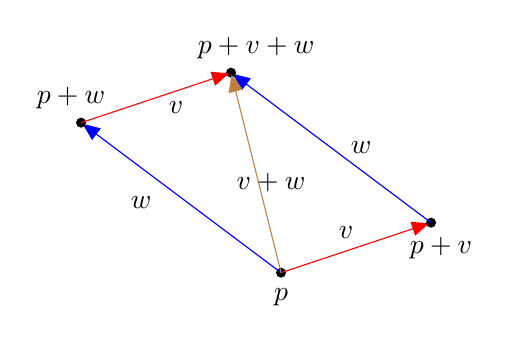
\begin{tikzpicture}[x=0.25in,y=0.25in]
\begin{scope}[>=triangle 45,shorten >=0.01in]

    \fill[black] (0,0) circle(0.1) + (+0.0,-0.5) node[black]{$p$};

    \draw[red,->] (0,0) -- (+3,+1);
    \draw[black] (1.3,0.8) node{$v$};
    \fill[black] (+3,+1) circle(0.1) + (+0.2,-0.5) node[black]{$p+v$};
    \draw[blue,->] (+3,+1) -- (-1,+4);
    \draw[black] (+1.6,2.5) node{$w$};
    \fill[black] (-1,+4) circle(0.1) + (+0.5,+0.5) node[black]{$p+v+w$};

    \draw[blue,->] (0,0) -- (-4,+3);
    \draw[black] (-2.8,1.4) node{$w$};
    \fill[black] (-4,+3) circle(0.1) + (-0.2,+0.5) node[black]{$p+w$};
    \draw[red,->] (-4,+3) -- (-1,+4);
    \draw[black] (-2.1,3.3) node{$v$};

    \draw[brown,->] (0,0) -- (-1,+4);
    \draw[black] (-0.2,1.8) node{$v+w$};
\end{scope}
\end{tikzpicture}
\end{wrapfigure}
We will define the \key{vector sum} of vectors $v=(v_x,v_y)$ and
$w=(w_x,w_y)$ to be $v+w=(v_x+w_x,v_y+w_y)$.  If you
think of a point $p=(p_x,p_y)$ in the XY-plane as a vector,
you can associate a translation $\tau_v$ of the XY-plane
with the vector $v$ using the equation $\tau_v(p)=p+v$.  Then\\
\hspace*{0.2in}$\tau_w(\tau_v(p)) = p+v+w = \tau_{v+w}(p)$ \\
See the picture.
\\[1ex]
Vector sums are commutative, i.e.,  $v+w=w+v$, and associative,
i.e., $u+(v+w)=(u+v)+w$.
\end{minipage}

\bigskip

\begin{minipage}{\textwidth}\raggedright
\begin{wrapfigure}{r}{0.55\textwidth}
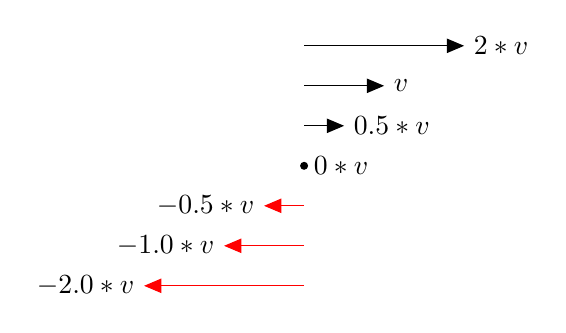
\begin{tikzpicture}[x=0.20in,y=0.20in]
\begin{scope}[>=triangle 45]

    \draw[black,->] (0,3) -- (4,3) node[black,right]{$2*v$};
    \draw[black,->] (0,2) -- (2,2) node[black,right]{$v$};
    \draw[black,->] (0,1) -- (1,1) node[black,right]{$0.5*v$};
    \fill[black] (0,0) circle(0.1) node[black,right]{$0*v$}; 
    \draw[red,->] (0,-1) -- (-1,-1) node[black,left]{$-0.5*v$};
    \draw[red,->] (0,-2) -- (-2,-2) node[black,left]{$-1.0*v$};
    \draw[red,->] (0,-3) -- (-4,-3) node[black,left]{$-2.0*v$};
\end{scope}
\end{tikzpicture}
\end{wrapfigure}
We define the \key{scalar product} of a scalar $s$ and a vector
$v=(v_x,v_y)$ as $s*v = (s*v_x,s*v_y)$.  Multiplication
of $v$ by $s>0$ does not change the direction of $v$,
but multiplies the length of $v$ by $s$.  Multiplication of $v$ by
$s<0$ reverses the direction of $v$ and multiplies its length
by $|s|$.  See the picture.
\\[1ex]
Scalar products are associative in that
$s_1*(s_2*v)=(s_1*s_2)*v$ and distributive in that
$s*(v_1+v_2)=s*v_1+s*v_2$ and $(s_1+s_2)*v = s_1*v + s_2*v$.
\end{minipage}

\medskip

The negative of a vector is defined as $-v = (-1)*v = (-v_x,-v_y)$.
Subtraction of vectors is defined as $v-w = v + (-w) = (v_x-w_x,v_y-w_y)$. 

\medskip

\begin{minipage}{\textwidth}\raggedright
\begin{wrapfigure}{r}{0.4\textwidth}
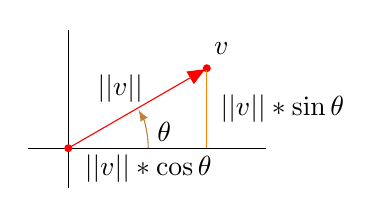
\begin{tikzpicture}[x=0.20in,y=0.20in]
\begin{scope}[>=triangle 45,shorten >=0.01in]
    \draw[black] (-1,0) -- (+5,0);
    \draw[black] (0,-1) -- (0,+3);

    \fill[red] (0,0) circle(0.1);
    \draw[black] (2.0,-0.5) node{$||v||*\cos \theta$};

    \draw[brown,>=latex,->] (2.0,0) arc(0:30:2.0);
    \draw[black] (2.4,+0.4) node{$\theta$};

    \fill[red] (3.464101615,2.0) circle(0.1);
    \draw[red,->] (0,0) -- (3.464101615,2.0);
    \draw[black] (1.3,+1.5) node{$||v||$};
    \draw[black] (3.4,+2.5) node[right]{$v$};

    \draw[orange] (3.464101615,0) -- (3.464101615,2.0);
    \draw[black] (3.464101615,1) + (0.1,0)
                 node[right]{$||v||*\sin \theta$};
\end{scope}
\end{tikzpicture}
\end{wrapfigure}
A vector $v=(v_x,v_y)$ has a length and a direction.
The \key{length}, denoted by $||v||$, can be computed using
Pythagoras's Theorem: $||v||=\sqrt{v_x^2+v_y^2}$.  The
direction is given by the counterclockwise angle $\theta$ from
the positive X-axis direction to the vector direction.
This is called the \key{azimuth} of $v$, and in computer
languages may be computed (in radians) by the {\tt atan2} function as
$\theta = \mathrm{atan2}(v_y,v_x)$ (note $v_y$ comes before $v_x$).
\end{minipage}

We measure angles, including azimuths, in degrees.  To convert degrees
to radians, multiply by $\pi/180$, and to convert radians to degrees,
multiply by $180/\pi$.  Positive angles are counter-clockwise, and
negative angles are clockwise.

For a vector {\tt v},~~{\tt azm v} and {\tt ||v||} are said to be
the \key{polar coordinates} of {\tt v}.
The vector with the polar coordinates $\theta$ (azimuth) and $\ell$ (length) is
$(\ell \cos\theta,\ell \sin\theta)$.
See the picture.

Adding integer multiples of 360 to a vector's
azimuth does \underline{not} change the vector.

\newpage

\section{Vector Calculator}
Implement additions to the basic calculator for just {\em vector}
value types and the {\em operators} and {\em functions}:
\begin{center}
\begin{tabular}{l@{~~~~~}l@{~~~~~}l}
Assume: & {\tt s=}$s$, {\tt x=}$x$, {\tt y=$y$},
          {\tt l=$\ell$}, {\tt t=$(180/\pi)*\theta$}
          are scalars \\
	& {\tt d=}$d$ (an integer scalar $0\le d\le 12$) \\
	& {\tt v=}$(v_x,v_y)$, {\tt w=}$(w_x,w_y)$ are vectors \\
then: \\[1ex]
\tt (x,y) & returns $(x,y)$ \\
\tt v.x & returns $v_x$ ~~~ ({\tt x} is \underline{not} a variable here) \\
\tt v.y & returns $v_y$ ~~~ ({\tt y} is \underline{not} a variable here) \\
\tt v==w:d & returns $v_x==w_x:d$ AND $v_y==w_y:d$ \\
\tt s*v & returns $(s v_x, s v_y )$ \\
\tt -v & returns $( -v_x, -v_y )$, {\tt v} with direction reversed \\
\tt v+w & returns $(v_x + w_x, v_y + w_y)$ \\
\tt v-w & returns $(v_x - w_x, v_y - w_y)$ \\
\tt ||v|| & returns $\sqrt{v_x^2 + v_y^2}$ & [length] \\
\tt azm v & returns $\mathrm{atan2}(v_y,v_x)*(180/\pi)$ & [azimuth] \\
\tt l\textasciicircum t
          & returns $(\ell\cos\theta,\ell\sin\theta)$, \\
	  & the vector with length {\tt l} and azimuth {\tt t} degrees \\
	  & where $\theta = (\pi/180)*{\tt t}$ radians \\
\end{tabular}
\end{center}

If {\tt ||v|| = 0} then {\tt azm~v} is undefined (you can do extra
programming to make it defined as {\tt nan} if you like, but this
is not necessary).

\begin{center}
\begin{tabular}{rl}
Sample Input Files: & \file{00-XXXX-vector-vec-2d.in} \\
Sample Output Files: & \file{00-XXXX-vector-vec-2d.ftest} \\
Sample Run File: & \file{sample-vector-vec-2d.run} \\
Submit Run File: & \file{submit-vector-vec-2d.run} \\
\end{tabular}
\end{center}

You can test your program using the indicated sample input and
output and you can submit your program using the indicated submit
run file.

\newpage

\section{Display Language}
Points, lines, arrows, etc.~can be displayed in a PDF file
by making a {\tt .pdf} file from an {\tt .in}
file and your solution program.
The display commands are embedded in {\tt .in} file `{\tt \#}' comment
lines, so your program does not have to deal with them.
The {\tt 00-001-vector-vec-2d.in} file has display commands,
but many {\tt .in} files have none.

\medskip

\begin{minipage}{\textwidth}
The line/area drawing commands are:
\\[1ex]
\begin{tabular}{@{}l@{~~~~~}l@{}}
\underline{Command} & \underline{Draws}
\\[1ex]
\tt \#!point p [color] [size] & point {\tt p} \\
\tt \#!point L [color] [size] & points in the point list {\tt L} \\
\tt \#!line pq [color] [opt] & line from point {\tt p}
                                 to point {\tt q} \\
\tt \#!line L  [color] [opt] & lines with endpoints that are \\
                             & consecutive points in the \\
		             & list of points {\tt L} \\
\tt \#!infline pA [color] [opt] & infinite line from point {\tt p} \\
                                & in direction {\tt A} and/or {\tt -A} \\
\tt \#!rectangle pq [color] [opt] & rectangle with opposing corners \\
                                  & point {\tt p} and point {\tt q} \\
\tt \#!circle cr [color] [opt] & circle of center {\tt c}
                                   and radius {\tt r} \\
\tt \#!ellipse cRA [color] [opt] & ellipse with center {\tt c}, radii \\
                                   & {\tt R.x} and {\tt R.y}, rotated \\
                                   & by angle A about its center \\
\end{tabular}
\end{minipage}

In the above {\tt p}, {\tt q}, {\tt c}, {\tt R}, {\tt r}, {\tt A}, {\tt L}
are arbitrary {\em variables}.
Circle and ellipse radii must be strictly positive.
Spaces are as indicated, and must consist
of at least one horizonal space character.

Coordinates are automatically scaled to fit the page.  Angles are
in degrees.

The possible colors
are `{\tt red}', `{\tt blue}', `{\tt brown}', and `{\tt black}'.  Black is
the default.
(Green does not show up when the page is printed in black-and-white, and
so is not provided.)

For points, {\tt size} is an integer in the range [1,18] giving the size
of each point in units of 1/72'nd inch (1pt).  The default is 2pt.

\begin{minipage}{\textwidth}
For non-points {\tt opt} is zero or more of:
\\[1ex]
\hspace*{0.5in}\begin{tabular}{rl}
    \tt . & dotted line \\
    \tt - & dashed line \\
          & ~~ ({\tt .} and {\tt -} conflict; if neither line is solid) \\
    \tt c & close path (for {\tt \#!line}) \\
          & ~~ (implied by {\tt s}, {\tt d}, {\tt h}, {\tt v}) \\
    \tt m & add arrow head in middle of each line segment (for {\tt \#!line}) \\
    \tt e & add arrow head at end of each line segment (for {\tt \#!line}) \\
    \tt s & fill with solid color \\
    \tt d & fill with dots \\
    \tt h & fill with horizontal bars \\
    \tt v & fill with vertical bars \\
          & ~~ ({\tt s}, {\tt d}, {\tt h}, and {\tt v} conflict) \\
    \tt f & extend infinite line forward from point \\
    \tt b & extend infinite line backward from point \\
          & ~~ ({\tt f}, {\tt b} conflict; if neither
	        line extends in both directions) \\
    \end{tabular}
\end{minipage}

\begin{minipage}{\textwidth}
The text drawing commands are:
\\[1ex]
\begin{tabular}{@{}l@{~~~~~}l@{}}
\underline{Command} & \underline{Draws}
\\[1ex]
\tt \#!text p [color] opt text... &
    the text, place at/near point {\tt p} \\
\tt \#!text pq [color] opt text... &
    ditto but the text is placed at/near \\
    & the midpoint of the line {\tt pq}
\end{tabular}
\end{minipage}

\begin{minipage}{\textwidth}
Here {\tt opt} is `{\tt -}' for no options, or given that the point
of text placement is {\tt ($x$,$y$)}, is one or more of:
\\[1ex]
\hspace*{0.5in}\begin{tabular}{rl}
    \tt t & display about 0.5em above $y$ \\
    \tt b & display about 0.5em below $y$ \\
          & ~~ ({\tt t} and {\tt b} conflict, if neither center on $y$) \\
    \tt l & display about 0.5em left of $x$ \\
    \tt r & display about 0.5em right of $x$ \\
          & ~~ ({\tt l} and {\tt r} conflict, if neither center on $x$) \\
    \tt x & make the bounding box of text white \\
    \tt c & make the bounding circle of text white \\
          & ~~ ({\tt x} and {\tt c} conflict) \\
    \tt o & outline any bounding box or circle with \\
          & a black line of width 1pt \\
    \end{tabular}
\end{minipage}


\begin{minipage}{\textwidth}
The page commands are:
\\[1ex]
\begin{tabular}{@{}l@{~~~~~}l@{~~~~~}l@{}}
\underline{Command} & \underline{Action}
\\[1ex]
\tt \#!layout R C [margin]   & Starts new physical page with R rows and \\
                             & C columns of logical pages, each logical \\
			     & page with margins as given in pt (1/72") \\
			     & (margin defaults to 18 or 0.25") \\
\tt \#!newpage [text...] & Starts new logical page \\
                         & with text line in page header \\
\tt \#!header text... & Adds text line to current page header \\
\end{tabular}
\end{minipage}

The output from a test case is one or more physical pages
each containing one or more logical pages.  The physical
pages are numbered and labelled with the test case name
(e.g., {\tt 00-000-vec-2d}).  Each `{\tt text...}' adds one
line to the logical page header.  If the first command is
not a `{\tt \#!layout}' command, then `{\tt \#!layout 1 1}'
is assumed.  A `{\tt \#!newpage}' command immediately after a
`{\tt \#!layout}' command may be omitted and will be assumed.

\newpage

\section{Linear Transforms}
If we let $\mathcal{R}$ denote the set of real numbers,
a.k.a., scalars, the set of all vectors is \\
\centerline{
$\mathcal{R}\times\mathcal{R}=\mathcal{R}^2
    =\{(v_x,v_y)|v_x,v_y\in \mathcal{R}\}$}

\begin{definition}\label{LINEAR-TRANSFORMATION}
A \key{linear transformation} $L$ is a continuous map
$L:\mathcal{R}^2\mapsto\mathcal{R}^2$ such that for
all vectors $v$ and $w$, $L(v+w)=L(v)+L(w)$.
\end{definition}

Some examples of linear transformations are (1) the identity map,
(2) rotations, (3) reflections about an axis, (4) scale changes
(i.e., $(v_x,v_y)\longmapsto(s_x v_x,s_y v_y)$ for scalars $s_x$
and $s_y$).

(In vector algebra, linear transformations with domains and/or ranges
that are vector spaces other than $\mathcal{R}^2$ are studied.)


\begin{lemma}
Let $L$ be a linear transformation, $v$ and $w$ be vectors,
and $0=(0,0)$ be the zero vector.  Then $L(0)=0$,  $L(-v)=-L(v)$,
and $L(v-w) = L(v) - L(w)$.
\end{lemma}
\begin{indpar}{0.5in}
Proof: $L(0) = L(0+0)= L(0) + L(0)$ so subtracting $L(0)$
from both sides, $0=L(0)$.  $0 = L(0) = L(v-v) = L(v) + L(-v)$
so subtracting $L(v)$ from both sides, $-L(v)=L(-v)$.
$L(v-w)=L(v+(-w))=L(v)+L(-w)=L(v)+(-L(w))=L(v)-L(w)$.
\end{indpar}

\begin{lemma}
Let $L$ be a linear transformation, $s$ be a scalar, and $v$ be a vector.
Then $L(s*v)=s*L(v)$.
\end{lemma}
\begin{indpar}{0.5in}
Proof: The cases $s=0,1,2,-1,-2$ follow from the previous lemma and
using induction proves the lemma for any integer $s$.  For $s=n/d$
a rational number with integers $n$ and $d$ and $d>0$, \\
\hspace*{0.1in}$n*L(v) = L(n*(d/d)*v) = L(d*(n/d)*v)=d*L((n/d)*v)$ \\
so dividing by $d$
we get $L((n/d)*v)=(n/d)*L(v)$.  For $s$ a non-rational real number,
the result follows from a continuity argument that we will leave
to the mathematicians, since computer scientists only compute
with rational numbers.
\end{indpar}

Let $L$ be a linear transformation; let $v=(v_x,v_y)$ be a vector;
let $u_x=(1,0)$ and $u_y =(0,1)$.  Then \\
\centerline{$L(v) = L(v_x*u_x+v_y*u_y)=v_x*L(u_x)+v_y*L(u_y)$.}

\begin{lemma}
Given vectors $\ell_x$ and $\ell_y$, the map
$L:(v_x,v_y)\longmapsto v_x*\ell_x+v_y*\ell_y$ is a linear
transformation.
\end{lemma}
\begin{indpar}{0.5in}
Proof: $L(v+w) = (v_x+w_x)*\ell_x+(v_y+w_y)*\ell_y
               = v_x*\ell_x+v_y*\ell_y+w_x*\ell_x+w_y*\ell_y
	       = L(v) + L(w)$.
\end{indpar}

So $L$ is determined by $\ell_x = L(u_x)$ and $\ell_y = L(u_y)$,
and there is a 1-1 correspondence between linear transformations
and vector pairs $[\ell_x,\ell_y]$.  Therefore we will represent a linear
transformation $L$ by a pair of vectors {\tt [$\ell_x$,$\ell_y$]}
and represent application of L to the vector {\tt v = ($v_x$,$v_y$)} by \\
\centerline{\tt $L(v)$ = [$\ell_x$,$\ell_y$]*($v_x$,$v_y$) =
             $v_x$*$\ell_x$+$v_y$*$\ell_y$}
Here we use [] instead of () to surround the pair of vectors of a linear
transformation, because our calculator does this to distinguish linear
transformations from lists of vectors.

Examples:
\begin{enumerate}
\item {\tt L=[(1,0),(0,1)]} is the identity map.
$L(v)=v_x*(1,0) + v_y*(0,1) = (v_x,0)+(0,v_y) = (v_x,v_y) = v$.
\item {\tt L=[(0,1),(-1,0)]} rotates vectors $90^\circ$.
Specifically, $L(u_x)=u_y$ and $L(u_y)=-u_x$ and
$L(v)=v_x*(0,1) + v_y*(-1,0) = (0,v_x)+(-v_y,0) = (-v_y,v_x)$.
\item {\tt L=[(-1,0),(0,-1)]} reverses the direction of a vector.
$L(v)=v_x*(-1,0) + v_y*(0,-1) = (-v_x,0)+(0,-v_y) = (-v_x,-v_y) = -v$.
\item {\tt L=[(-1,0),(0,1)]} reflects vectors across the Y-axis.
$L(v)=v_x*(-1,0) + v_y*(0,1) = (-v_x,0)+(0,v_y) = (-v_x,v_y)$.
\item {\tt L=[($s_x$,0),(0,$s_y$)]} scales the X-axis by $s_x$ and
the Y-axis by $s_y$. \\
$L(v)=v_x*(s_x,0) + v_y*(0,s_y)
     = (s_x v_x,0)+(0,s_y v_y)= (s_x v_x, s_y v_y)$.
\end{enumerate}

Now suppose we have a scalar {\tt s}, vector {\tt v},
and two linear transformations
{\tt K = [$\ell^K_x$,$\ell^K_y$]},
{\tt L = [$\ell^L_x$,$\ell^L_y$]}.  Then we can define:
\begin{center}
\tt
\begin{tabular}{l@{~so that~}l}
s*L = [s*$\ell^L_x$,s*$\ell^L_y$]
	 & (s*L)*v = s*(L*v) \\[0.3ex]
K+L = [$\ell^K_x$+$\ell^L_x$,$\ell^K_y$+$\ell^L_y$]
	 & (K+L)*v = K*v + L*v \\[0.3ex]
K-L = [$\ell^K_x$-$\ell^L_x$,$\ell^K_y$-$\ell^L_y$]
	 & (K-L)*v = K*v - L*v \\[0.3ex]
-L = [-$\ell^L_x$,-$\ell^L_y$]
	 & (-L)*v = - L*v \\[0.3ex]
K*L = [K*$\ell^L_x$,K*$\ell^L_y$]
	 & (K*L)*v = K*(L*v)
\end{tabular}
\end{center}

{\tt *} and {\tt +} as defined here are \key{bi-linear}, which means
(letting {\tt J} be another linear transformation):
\begin{center}
\tt
s*(K+L) = s*K + s*L \\
(J+K)*L = J*L + K*L \\
J*(K+L) = J*K + J*L
\end{center}

Addition of linear transformations commutes,
{\tt K+L = L+K}, but multiplication does not:
in general {\tt K*L} is \underline{not equal} to {\tt L*K}
(as an example, a rotation does not generally commute with
a reflection: see the end of the Rotations and Reflections
section below).

Let {\tt I} be the identity transform defined by
{\tt I*v=v} for all vectors {\tt v}  (and therefore {\tt I=[$u_x$,$u_y$]}).
It is easy to check that {\tt K*I = K = I*K} for all linear transforms
{\tt K}.

A linear transform {\tt K} is defined to be the (two-sided) \key{inverse}
of the linear transform {\tt L} if and only if {\tt K*L = I = L*K}.
The inverse of {\tt L} might not exist, but if it does, it is unique
since if there were two, {\tt K$_1$} and {\tt K$_2$}, then \\
\centerline{\tt K$_1$ = K$_1$*I = K$_1$*(L*K$_2$)
                      = (K$_1$*L)*K$_2$ = I*K$_2$ = K$_2$}
The notation {\tt L$^{-1}$} is used for the inverse of {\tt L} if it
exists.  For example, the inverse of a rotation by angle $\phi$ in the
counter-clockwise direction is a rotation by angle $\phi$ in the
clockwise direction.

(One-sided inverses that are not two-sided inverses only exist for
linear transformations whose domain and range are vector spaces of
\underline{different} dimensions, unlike our linear transformations
whose domain and range are both 2-dimensional.)



\newpage

\section{Linear Transform Calculator}
Implement additions to the vector calculator for just {\em linear-transform}
value types and the {\em operators} and {\em functions}:
\begin{center}
\begin{tabular}{l@{~~~~~}l@{~~~~~}l}
Assume: & {\tt s=}$s$ is a scalar \\
	& {\tt d=}$d$ (an integer scalar $0\le d\le 12$) \\
	& {\tt v=($v_x$,$v_y$)} and {\tt w=($w_x$,$w_y$)} are vectors \\
	& \multicolumn{2}{@{}l}{{\tt K=[$\ell^K_x$,$\ell^K_y$]} and
	  {\tt L=[$\ell^L_x$,$\ell^L_y$]} are linear transforms} \\
then: \\[1ex]
\tt (v,w) & returns $(v,w)$ \\
\tt K==L:d & returns $\ell^K_x==\ell^L_x:d$ AND $\ell^K_y==\ell^L_y:d$ \\
\tt L.x & returns {\tt $\ell^L_x$}
          ~~~ ({\tt x} is \underline{not} a variable here) \\
\tt L.y & returns {\tt $\ell^L_y$}
          ~~~ ({\tt y} is \underline{not} a variable here) \\
\tt L*v & returns {\tt $v_x$*$\ell^L_x$+$v_y$*$\ell^L_y$} & [application] \\
\tt s*L & returns {\tt [$s\ell^L_x$,$s\ell^L_y$]} \\
\tt K+L & returns {\tt [$\ell^K_x$+$\ell^L_x$,$\ell^K_y$+$\ell^L_y$]} \\
\tt K-L & returns {\tt [$\ell^K_x$-$\ell^L_x$,$\ell^K_y$-$\ell^L_y$]} \\
\tt -L & returns {\tt [-$\ell^L_x$,-$\ell^L_y$]} \\
\tt K*L & returns {\tt [K*$\ell^L_x$,K*$\ell^L_y$]} & [composition] \\
\end{tabular}
\end{center}

\begin{center}
\begin{tabular}{rl}
Sample Input Files: & \file{00-XXXX-linear-vec-2d.in} \\
Sample Output Files: & \file{00-XXXX-linear-vec-2d.ftest} \\
Sample Run File: & \file{sample-linear-vec-2d.run} \\
Submit Run File: & \file{submit-linear-vec-2d.run} \\
\end{tabular}
\end{center}

\newpage

\section{Rotations and Reflections}
Rotations and reflections are the two kinds of linear transformations
that preserve vector lengths (i.e., $||L(v)||=||v||$).

\begin{minipage}{\textwidth}\raggedright
\begin{wrapfigure}[5]{r}{0.4\textwidth}
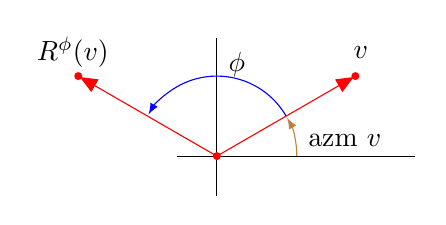
\begin{tikzpicture}[x=0.20in,y=0.20in]
\begin{scope}[>=triangle 45,shorten >=0.01in]
    \draw[black] (-1,0) -- (+5,0);
    \draw[black] (0,-1) -- (0,+3);

    \fill[red] (0,0) circle(0.1);

    \draw[brown,>=latex,->] (2.0,0) arc(0:30:2.0);
    \draw[black] (3.2,+0.4) node{azm~$v$};

    \draw[blue,>=latex,->] (1.7320508,1.0) arc(30:150:2.0);
    \draw[black] (+0.5,+2.3) node{$\phi$};

    \fill[red] (3.464101615,2.0) circle(0.1);
    \draw[red,->] (0,0) -- (3.464101615,2.0);
    \draw[black] (3.6,2.6) node{$v$};

    \fill[red] (-3.464101615,2.0) circle(0.1);
    \draw[red,->] (0,0) -- (-3.464101615,2.0);
    \draw[black] (-3.6,+2.6) node{$R^\phi(v)$};

\end{scope}
\end{tikzpicture}
\end{wrapfigure}
A \key{rotation} $R^\phi$ by $\phi$ degrees (counter-\EOL clockwise)
is defined mathematically by
\hspace*{0.2in}\begin{tabular}[t]{l}
$||R^\phi(v)|| = ||v||$ \\
$\mathrm{azm}~R^\phi(v) = \mathrm{azm}~v + \phi$ \\
\end{tabular} \\
~\\
A rotation preserves angles between vectors; that is: \\
\hspace*{0.2in}$\mathrm{azm}~R^\phi(v)-\mathrm{azm}R^\phi(w)
               = \mathrm{azm}~v-\mathrm{azm}~w$ \\
Also, adding integer multiples of 360 to $\phi$
does \underline{not} change $R^\phi$.
\end{minipage}

\bigskip

\begin{minipage}{\textwidth}\raggedright
\begin{wrapfigure}[5]{r}{0.5\textwidth}
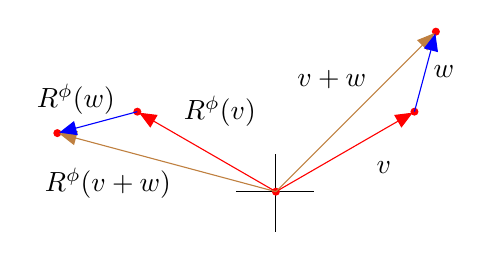
\begin{tikzpicture}[x=0.20in,y=0.20in]
\begin{scope}[>=triangle 45,shorten >=0.01in]
    \draw[black] (-1,0) -- (+1,0);
    \draw[black] (0,-1) -- (0,+1);

    \fill[red] (0,0) circle(0.1);

    \fill[red] (3.464101615,2.0) circle(0.1);
    \draw[red,->] (0,0) -- (3.464101615,2.0);
    \draw[black] (2.7,0.6) node{$v$};

    \fill[red] (4.0,4.0) circle(0.1);
    \draw[brown,->] (0,0) -- (4.0,4.0);
    \draw[black] (1.4,2.8) node{$v+w$};

    \draw[blue,->] (3.464101615,2.0) -- (4.0,4.0);
    \draw[black] (4.2,3.0) node{$w$};

    \fill[red] (-3.464101615,2.0) circle(0.1);
    \draw[red,->] (0,0) -- (-3.464101615,2.0);
    \draw[black] (-1.4,+2.0) node{$R^\phi(v)$};

    \fill[red] (-5.464101521,1.464101590) circle(0.1);
    \draw[brown,->] (0,0) -- (-5.464101521,1.464101590);
    \draw[black] (-4.2,+0.2) node{$R^\phi(v+w)$};

    \draw[blue,->] (-3.464101615,2.0) -- (-5.464101521,1.464101590);
    \draw[black] (-5.0,2.3) node{$R^\phi(w)$};

\end{scope}
\end{tikzpicture}
\end{wrapfigure}
A rotation perserves side-lengths and angles of a triangle.
Therefore, a rotation preserves vector addition, that is,
$R^\phi(v+w)=R^\phi(v)+R^\phi(w)$, and thus
satisfies Definition~\ref{LINEAR-TRANSFORMATION}
and is a linear transformation.
\end{minipage}

\bigskip

\begin{minipage}{\textwidth}\raggedright
\begin{wrapfigure}[6]{r}{0.4\textwidth}
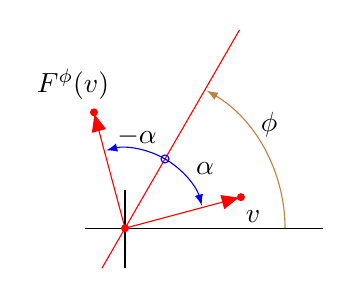
\begin{tikzpicture}[x=0.20in,y=0.20in]
\begin{scope}[>=triangle 45,shorten >=0.01in]
    \draw[black] (-1,0) -- (+5,0);
    \draw[black] (0,-1) -- (0,+1);

    \fill[red] (0,0) circle(0.1);

    \draw[red] (-0.577350269,-1) -- (2.886751345,5);

    \draw[brown,>=latex,->] (4.0,0) arc(0:60:4.0);
    \draw[black] (3.6,2.6) node{$\phi$};

    \fill[red] (2.897777478,0.776457135) circle(0.1);
    \draw[red,->] (0,0) -- (2.897777478,0.776457135);
    \draw[black] (3.2,0.3) node{$v$};

    \fill[red] (-0.776457135,2.897777478) circle(0.1);
    \draw[red,->] (0,0) -- (-0.776457135,2.897777478);
    \draw[black] (-1.3,+3.6) node{$F^\phi(v)$};

    \draw[blue,>=latex,->] (1.0,1.732050807) arc(60:15:2.0);
    \draw[black] (2.0,1.5) node{$\alpha$};

    \draw[blue] (1.0,1.732050807) circle(0.1);

    \draw[blue,>=latex,->] (1.0,1.732050807) arc(60:105:2.0);
    \draw[black] (0.3,2.3) node{$-\alpha$};

\end{scope}
\end{tikzpicture}
\end{wrapfigure}
A \key{reflection} $F^\phi$ by $\phi$ degrees, which
is a reflection across the line with direction $\phi$
through the origin,
is defined mathematically by
\hspace*{0.2in}\begin{tabular}[t]{l}
$||F^\phi(v)|| = ||v||$ \\
$\mathrm{azm}~F^\phi(v) = \phi - \alpha$ \\
where $\alpha = \mathrm{azm}~v - \phi$ so \\
$\mathrm{azm}~F^\phi(v) = 2*\phi - \mathrm{azm}~v$ \\
\end{tabular} \\
~\\
A reflection negates angles between vectors; that is: \\
\hspace*{0.2in}$\mathrm{azm}~F^\phi(v)-\mathrm{azm}F^\phi(w)
               = -(\mathrm{azm}~v-\mathrm{azm}~w)$ \\
Also, adding integer multiples of 180 to $\phi$
does \underline{not} change $F^\phi$.
\end{minipage}

\bigskip

\begin{minipage}{\textwidth}\raggedright
\begin{wrapfigure}[7]{r}{0.5\textwidth}
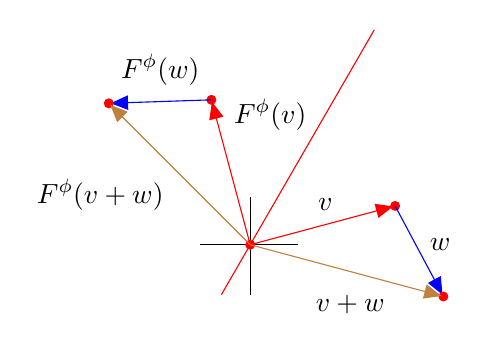
\begin{tikzpicture}[x=0.25in,y=0.25in]
\begin{scope}[>=triangle 45,shorten >=0.01in]
    \draw[black] (-1,0) -- (+1,0);
    \draw[black] (0,-1) -- (0,+1);

    \fill[red] (0,0) circle(0.1);

    \draw[red] (-0.577350269,-1) -- (2.5,4.330127018);

    \fill[red] (2.897777478,0.776457135) circle(0.1);
    \draw[red,->] (0,0) -- (2.897777478,0.776457135);
    \draw[black] (1.5,0.8) node{$v$};

    \draw[blue,->] (2.897777478,0.776457135) -- (3.863703305,-1.035276180);
    \draw[black] (3.8,-0.0) node{$w$};

    \fill[red] (3.863703305,-1.035276180) circle(0.1);
    \draw[brown,->] (0,0) -- (3.863703305,-1.035276180);
    \draw[black] (2.0,-1.2) node{$v+w$};

    \fill[red] (-0.776457135,2.897777478) circle(0.1);
    \draw[red,->] (0,0) -- (-0.776457135,2.897777478);
    \draw[black] (+0.4,+2.6) node{$F^\phi(v)$};

    \draw[blue,->] (-0.776457135,2.897777478) -- (-2.828427124,2.828427124);
    \draw[black] (-1.8,+3.5) node{$F^\phi(w)$};

    \fill[red] (-2.828427124,2.828427124) circle(0.1);
    \draw[brown,->] (0,0) -- (-2.828427124,2.828427124);
    \draw[black] (-3.0,+1.0) node{$F^\phi(v+w)$};

\end{scope}
\end{tikzpicture}
\end{wrapfigure}
A reflection perserves side-lengths and negates angles of a triangle.
Therefore, a reflection preserves vector addition, that is,
$F^\phi(v+w)=F^\phi(v)+F^\phi(w)$, and thus
satisfies Definition~\ref{LINEAR-TRANSFORMATION}
and is a linear transformation.
\end{minipage}

\vspace{0.5in}

A linear map $L$ that preserves vector lengths ($||L(v)||=||v||$)
is said to be \key{unitary}.
A unitary linear map $L$
also preserves the absolute values of angles between vectors,
because $L$ preserves the side-lengths of any triangle made of
vectors, and these determine the absolute values of the angles of
the triangle (but not the direction of these angles).  This means
that {\tt azm L(v)} must be either `{\tt {\rm constant} + azm v}'
or `{\tt {\rm constant} - azm v}'.  These two case are rotations
and reflections, respectively.

Now
$L$, being linear, is determined by $L(u_x)$ and $L(u_y)$, where
$u_x=(1,0)$ and $u_y=(0,1)$, and as $u_y$ is perpendicular to
$u_x$, $L(u_y)$ must be perpendicular to $L(u_x)$ since $L$ is unitary.

Putting all this together we have:
\begin{lemma}
For unitary $L=[\ell_x,\ell_y]$, $\ell_x$ and $\ell_y$ are
vectors of unit length, and $\ell_y$ is perpendicular to $\ell_u$.

If $\ell_y$ is $\ell_x$ rotated counter-clockwise
by 90 degrees, $L$ is a rotation, whereas if
$\ell_y$ is $\ell_x$ rotated clockwise
by 90 degrees, $L$ is a reflection.
\end{lemma}

If $L$ is a rotation, the angle of rotation is: \\
\centerline{$\phi = \mathrm{azm}~L(u_x) - \mathrm{azm}~u_x =
             \mathrm{azm}~L(u_x)$}
and we have: \begin{tabular}[t]{l}
             $L(u_x)=(\cos\phi,\sin\phi)$ \\
             $L(u_y)=(-\sin\phi,\cos\phi)$ \\
	     \end{tabular}

If $L$ is a reflection, the angle of the reflecting line is: \\
\centerline{$\phi = (1/2)*(\mathrm{azm}~L(u_x) + \mathrm{azm}~u_x)
                  = (1/2)*(\mathrm{azm}~L(u_x))$}
and we have: \begin{tabular}[t]{l}
             $L(u_x)=(\cos(2*\phi),\sin(2*\phi))$ \\
             $L(u_y)=(\sin(2*\phi),-\cos(2*\phi))$ \\
	     \end{tabular}

Both rotations and reflections preserve vector lengths
and change vector angles according to a linear formula.
Using the notation $R^\phi$ for rotation by angle $\phi$,
and $F^\phi$ for reflection about the line at angle $\phi$,
we get the following:
\begin{center}
$R^\phi*R^\omega=R^\omega*R^\phi=R^{\phi+\omega}$
~~because~~
    $(\mathrm{azm}~v + \omega) + \phi = \mathrm{azm}~v + (\phi+\omega)$ \\
$F^\phi*F^\omega = R^{2(\phi-\omega)}$
~~because~~
    $2\phi - (2\omega - \mathrm{azm}~v) = \mathrm{azm}~v + 2(\phi-\omega)$ \\
$R^\phi*F^\omega = F^\omega*R^{-\phi}$
~~because~~
    $(2\omega - \mathrm{azm}~v) + \phi =
      2\omega - (\mathrm{azm}~v + (-\phi))$
\end{center}
Note that:
\begin{center}
$R^\phi*R^\omega=R^{\omega+\phi}=R^\omega*R^\phi$ \\
$R^\phi$ and $R^\omega$ commute \\
$R^{-\phi}$ is the inverse of $R^\phi$ \\
$F^\phi*F^\phi= I$ (the identity) so  $F^\phi$ is its own inverse \\
$F^\omega*F^\phi$ is the inverse of $F^\phi*F^\omega$ \\
in general $F^\phi$ and $F^\omega$ do \underline{not} commute\\
\end{center}

\bigskip

\section{Rotations and Reflections Calculator}
Implement additions to the linear calculator for
the {\em operators} and {\em functions}:
\begin{center}
\begin{tabular}{l@{~~~~~}l@{~~~~~}l}
\multicolumn{2}{l}{Assume:} \\
        & {\tt p} is a scalar \\
	& {\tt v} is a vector \\
then: \\[1ex]
\tt v\textasciicircum p & returns {\tt w} such that {\tt ||w||=||v||} and
	                  {\tt azm w = azm v + p}, \\
			& {\tt v} rotated by {\tt p} degrees \\
\tt v|p & returns {\tt w} such that {\tt ||w||=||v||} and
	                  {\tt azm w = 2*p\,-\,azm v}, \\
			& {\tt v} reflected across the line with direction
			  {\tt p} degrees \\
\tt \textasciicircum p
       & returns {\tt ($u_x$\textasciicircum p,$u_y$\textasciicircum p)}, \\
       & the rotation $R^p$ with angle $p$ degrees \\
\tt |p & returns {\tt ($u_x$|p,$u_y$|p)}, \\
       & the reflection $F^p$ across the line with direction $p$ degrees \\
\end{tabular}
\end{center}

\begin{center}
\begin{tabular}{rl}
Sample Input Files: & \file{00-XXXX-unitary-vec-2d.in} \\
Sample Output Files: & \file{00-XXXX-unitary-vec-2d.ftest} \\
Sample Run File: & \file{sample-unitary-vec-2d.run} \\
Submit Run File: & \file{submit-unitary-vec-2d.run} \\
\end{tabular}
\end{center}

\newpage

\section{Products}
There are two products of a pair of vectors that play a
very important role in 2D computational geometry:

\begin{definition}
The \key{scalar product} of two vectors \\
\centerline{{\tt v = ($v_x$,$v_y$)} and {\tt w = ($w_x$,$w_y$)}} \\
is \\
\centerline{\tt v*w = $v_x w_x + v_y w_y$} \\
The \key{cross product} of the two vectors is \\
\centerline{\tt v\#w = $(-v_y)w_x + v_x w_y$}
\end{definition}

Note that {\tt ||v||$^2$ = v*v}.

If we denote the rotation counter-clockwise by 90 degrees by {\tt R}$^{90}$,
then \\
\centerline{\tt v\#w = (-$v_y$,$v_x$)*w = R$^{90}$(v)*w}

Both the scalar and cross product are \key{bi-linear}.  That is,
if {\tt u}, {\tt v}, {\tt w} are vectors and {\tt s} is a scalar:
\begin{center}
\tt
(u+v)*w = u*w + v*w \\
u*(v+w) = u*v + u*w \\
(s*u)*w = s*(u*w) = u*(s*w) \\
(u+v)\#w = u\#w + v\#w \\
u\#(v+w) = u\#v + u\#w \\
(s*u)\#w = s*(u\#w) = u\#(s*w)
\end{center}

The scalar product is symmetric ({\tt v*w = w*v})
while the cross product is anti-symmetric ({\tt v\#w = -w\#v}).

\begin{lemma}
For a unitary transform {\tt L}:
\begin{enumerate}
\item {\tt L(v)*L(w) = v*w} for all vectors {\tt v} and {\tt w}.
\item If {\tt L} is a rotation,
         {\tt L(v)\#L(w) = v\#w} for all vectors {\tt v} and {\tt w}; \\
      if {\tt L} is a reflection,
         {\tt L(v)\#L(w) = - v\#w} for all vectors {\tt v} and {\tt w}.
\end{enumerate}
\end{lemma}

\begin{indpar}{0.3in}
Proof: Since {\tt L} is unitary: \\
{\small \tt
\hspace*{0.05in}
       \begin{tabular}[t]{rcl}
       ||v+w||$^2$ & = & (v+w)*(v+w) = v*v + v*w + w*v + w*w \\
		   & = & ||v||$^2$ + 2*v*w + ||w||$^2${\rm ,} \\
       {\rm so} v*w & = & (1/2) \\
                    & * & ( ||v+w||$^2$ - ||v||$^2$ - ||w||$^2$ ){\rm ,} \\
       {\rm so} L(v)*L(w)
         & = & (1/2) \\
	 & * & (||L(v)+L(w)||$^2$-||L(v)||$^2$-||L(w)||$^2$) \\
         & = & (1/2)*( ||v+w||$^2$ - ||v||$^2$ - ||w||$^2$ ) \\
         & = & v*w
       \end{tabular}
} % \small \tt

If $L$ is a rotation, {\tt R$^{90}$*L=L*R$^{90}$} so \\
{\tt
\hspace*{0.1in}
       \begin{tabular}[t]{rcl}
       L(v)\#L(w) & = & R$^{90}$(L(v))*L(w) = L(R$^{90}$(v))*L(w) \\
                  & = & R$^{90}$(v)*w = v\#w \\
       \end{tabular}
} % \tt

If $L$ is a reflection, {\tt R$^{90}$*L=L*R$^{-90}$}
and {\tt R$^{-90}$ = - R$^{90}$} so \\
{\tt
\hspace*{0.1in}
       \begin{tabular}[t]{rcl}
       L(v)\#L(w) & = & R$^{90}$(L(v))*L(w) = L(R$^{-90}$(v))*L(w) \\
                  & = & R$^{-90}$(v)*w = - R$^{90}$(v)*w = - v\#w
       \end{tabular}
} % \tt
\end{indpar}


\bigskip

\begin{minipage}{\textwidth}\raggedright
\begin{wrapfigure}{r}{0.5\textwidth}
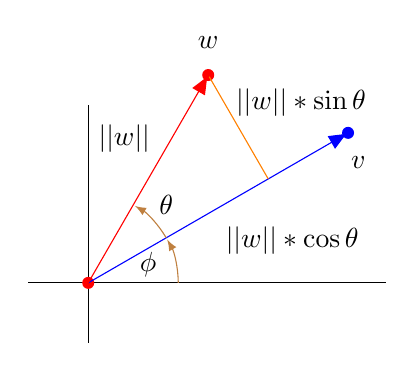
\begin{tikzpicture}[x=0.30in,y=0.30in]
\begin{scope}[>=triangle 45,shorten >=0.01in]
    \draw[black] (-1,0) -- (+5,0);
    \draw[black] (0,-1) -- (0,+3);
    \fill[red] (0,0) circle(0.1);

    \fill[blue] (4.330127018,2.5) circle(0.1);
    \draw[blue,->] (0,0) -- (4.330127018,2.5);
    \draw[black] (4.5,2.0) node{$v$};

    \fill[red] (2.0,3.464101615) circle(0.1);
    \draw[red,->] (0,0) -- (2.0,3.464101615);
    \draw[black] (0.6,+2.4) node{$||w||$};
    \draw[black] (2.0,+4.0) node{$w$};

    \draw[orange] (3.0,1.732050807) -- (2.0,3.464101615);
    \draw[black] (2.3,3.0) node[right]{$||w||*\sin \theta$};

    \draw[black] (3.4,0.7) node{$||w||*\cos \theta$};

    \draw[brown,>=latex,->] (1.5,0) arc(0:30:1.5);
    \draw[black] (1.0,+0.3) node{$\phi$};

    \draw[brown,>=latex,->] (1.299038105,0.75) arc(30:60:1.5);
    \draw[black] (1.3,+1.3) node{$\theta$};

\end{scope}
\end{tikzpicture}
\end{wrapfigure}
We can use the fact that $*$ and $\#$ are invariant under
rotations to give a geometric characterization
of these two products.  Let $v$ and $w$ be two vectors, let
$\theta=\mathrm{azm}~w - \mathrm{azm}~v$ be the direction angle of $w$
relative to $v$, and let $\phi = \mathrm{azm}~v$ be the aszimuth of $v$
(see the picture).
If we rotate both vectors by $R^{-\phi}$
we line $v$ up with the positive X-axis, while not changing $\theta$,
$||v||$, $||w||$, $v*w$, or $v\#w$.  So after rotation we have
\hspace*{0.5in}
    \begin{tabular}{l@{~~~~~}l}
    $v=(||v||,0)$ &
    $w=(||w||\cos\theta,||w||\sin\theta)$ \\
    $v*w=||v||\times||w||\times\cos\theta$ & 
    $v\#w=||v||\times||w||\times\sin\theta$ \\
    \end{tabular}
\end{minipage}

From this we deduce two things.  First, \\
\hspace*{0.5in}
    \begin{tabular}{l@{~~~~~}l}
    $v*w=||v||\times||w||\times\cos\theta$ &
    $v\#w=||v||\times||w||\times\sin\theta$ \\
    \end{tabular} \\
before rotation, as well as after rotation,
which gives a geometric characterization of the products.

Second,\hspace{0.5in}$||v||*R^{-\mathrm{azm}~v}*w=(v*w,v\#w)$,
\\[1ex]
which gives us a quick way to change coordinate systems
by a rotation times scalar multiplication by $||v||$ so that
$v$ has coordinates $(||v||^2,0)$ in the new coordinate system.
Problems that might be hard to solve in the original
coordinate system can be easly to solve in the new coordinate
system.  For example, the end of $w$ is to the left of the infinite directed
line extending $v$ if and only if $v\#w>0$.  One can also solve
distance problems in the original coordinate system by solving them
in the new coordinate system while remembering that the new system distances
are $||v||$ times the old system distances.

Note that a distance in
the new coordinate system is $||v||$ times the corresponding
distance in the old coordinate system.  If absolute distances are
of importance, it may be best to choose $v$ so that $||v||=1$.

\bigskip

\begin{minipage}{\textwidth}\raggedright
\begin{wrapfigure}{r}{0.37\textwidth}
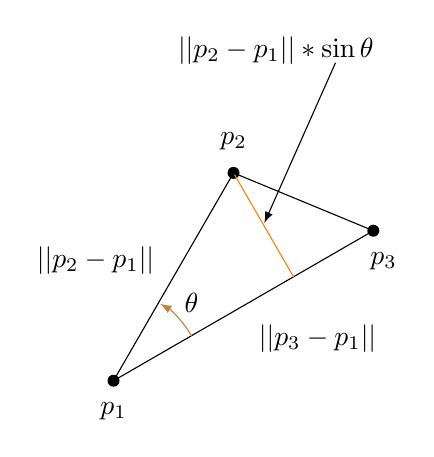
\begin{tikzpicture}[x=0.30in,y=0.30in]
\begin{scope}[>=triangle 45,shorten >=0.01in]

    \fill[black] (0,0) circle(0.1);
    \draw[black] (0.0,-0.5) node{$p_1$};

    \fill[black] (2.0,3.464101615) circle(0.1);
    \draw[black] (0,0) -- (2.0,3.464101615);
    \draw[black] (2.0,+4.0) node{$p_2$};
    \draw[black] (-0.3,+2.0) node{$||p_2-p_1||$};

    \fill[black] (4.330127018,2.5) circle(0.1);
    \draw[black] (2.0,3.464101615) -- (4.330127018,2.5);
    \draw[black] (4.5,2.0) node{$p_3$};

    \draw[black] (4.330127018,2.5) -- (0,0);

    \draw[orange] (3.0,1.732050807) -- (2.0,3.464101615);
    \draw[black] (4.5,5.5) node[left]{$||p_2-p_1||*\sin \theta$};
    \draw[black,>=latex,->] (3.7,5.3) -- (2.5,2.598076);

    \draw[black] (3.4,0.7) node{$||p_3-p_1||$};

    \draw[brown,>=latex,->] (1.299038105,0.75) arc(30:60:1.5);
    \draw[black] (1.3,+1.3) node{$\theta$};

\end{scope}
\end{tikzpicture}
\end{wrapfigure}
Lastly, looking at the picture at the right, we see that:
\hspace*{0.2in}
    \begin{tabular}{r@{~=~}l}
    \multicolumn{2}{l}{area of triangle $p_1 p_2 p_3$} \\
    & $(1/2)*||p_2-p_1||*\sin\theta*||p_3-p_1||$ \\
    & $(1/2)*(p_3-p_1)\#(p_2-p_1)$ \\
    & $-~(1/2)*(p_2-p_1)\#(p_3-p_1)$ \\
    \end{tabular} \\
~\\
So we can use the cross product to compute triangle areas,
but its a bit tricky because what we get is a signed area.
The result is positive if
the angle $\theta$ measured from the first factor of $\#$ to the
second factor of $\#$ is in the range $[0,180]$, and negative if
$\theta$ is in the range $[-180,0]$.
\end{minipage}

\newpage


\section{Products Calculator}
Implement additions to the unitary calculator for
the following {\em operators} and {\em functions}:
\begin{center}
\begin{tabular}{l@{~~~~~}l@{~~~~~}l}
Assume: & {\tt v=$v$=}$(v_x,v_y)$ (a vector)
          ~~~ {\tt w=$w$=}$(w_x,w_y)$ (a vector) \\
	& $u_x=(1,0)$ and $u_y=(0,1)$ \\
	& {\tt p=}$p$, {\tt q=}$q$, {\tt r=}$r$ (vectors representing points) \\
then: \\[1ex]
\tt v*w & returns $v_x w_x + w_y w_y$,
          the scalar product of {\tt v} and {\tt w} \\
\tt v\#w & returns $(-v_y)w_x+v_x w_y$,
           the cross product of {\tt v} and {\tt w} \\
\tt v:w & returns $||v||*R^{-\mathrm{azm}~v}*w = (v*w,v\#w)$ \\
\tt <v> & returns $(1/||v|)*v$, the unit vector in the same direction as $v$ \\
\tt v!w & returns $R^{-\mathrm{azm}~v}*w = (<v>*w,<v>\#w)$ \\
\tt v:  & returns {\tt [$v$:$u_x$,$v$:$u_y$]} ~~~ (so {\tt (v:)*w = v:w}) \\
\tt v!  & returns {\tt [$v$!$u_x$,$v$!$u_y$]} ~~~ (so {\tt (v!)*w = v!w}) \\
\tt area~pqr & returns $0.5*(r-p)\#(q-p)$, the area of triangle $pqr$, \\
             & with positive sign if $pqr$ clockwise, \\
	     & and negative sign if counter-clockwise \\
\end{tabular}
\end{center}

If {\tt ||v|| = 0} then {\tt <v>} and {\tt v!w} will produce coordinates such as
{\tt inf} (plus infinity), {\tt -inf} (minus infinity),
and {\tt nan} (not a number; i.e., result could not be computed).

\begin{center}
\begin{tabular}{rl}
Sample Input Files: & \file{00-XXXX-product-vec-2d.in} \\
Sample Output Files: & \file{00-XXXX-product-vec-2d.ftest} \\
Sample Run File: & \file{sample-product-vec-2d.run} \\
Submit Run File: & \file{submit-product-vec-2d.run} \\
\end{tabular}
\end{center}

\newpage

\section{Line and Point}\label{LINE-AND-POINT}
In this section we investigate the following questions:
\begin{enumerate}
\item Is a point on, to the left of, or to the right of
an infinite directed line?  What is the distance from the
point to the line and where is the closest point that is
on the line?
\item What is the general position of a point relative
to a finite line segment?  What is the distance from the
point to the line segment?
\end{enumerate}

We begin with a line {\tt pq} from point {\tt p} to point {\tt q},
{\tt p$\neq$q}.
We may take this line to be either infinite, or to be a finite
line seqment with ends {\tt p} and {\tt q}.  We may take the
line to be undirected, or to be directed from {\tt p} to {\tt q}.

We then consider a third point {\tt r} and ask about its relation
to {\tt pq}.

The answers to our questions will not be changed if we perform
a coordinate translation on all the points, so we begin by moving
{\tt p} to the origin {\tt (0,0)} using a translation by {\tt -p}.
Our points become:
\begin{center} \tt
p - p = (0,0) \\
q - p \\
r - p
\end{center}
Next we apply the rotation $R^{\tt -azm(q-p)}$
followed by multiplication by {\tt ||q-p||}.  This was computed
in the last section as the linear transform \\
\centerline{\tt (q-p): = ||q-p||*$R^{\tt -azm(q-p)}$}
This transformation preserves angles and multiplies distances by {\tt ||q-p||}.

If we apply {\tt (q-p):} after the translation {\tt -p}, we get:
\begin{center} \tt
P = (q-p):(p-p) = (0,0) \\
Q = (q-p):(q-p) = ( (q-p)*(q-p), 0 ) \\
R = (q-p):(r-p) = ( (q-p)*(r-p), (q-p)\#(r-p) )
\end{center}
where we use the facts that {\tt p - p = (0,0)} and
{\tt (q-p)\#(q-p) = 0}.

Next we define {\tt X} and {\tt Y} to be the coordinates of {\tt R}
so {\tt R = (X,Y)}, and {\tt L} to be the X coordinate of {\tt Q}
so {\tt Q = (L,0)}.

If\label{DISTANCE-OF-LINE-TO-POINT}
we want the distance from {\tt r} to the infinite line {\tt pq},
then this is the same as {\tt 1/||q-p||} times
the distance from {\tt R = (X,Y)} to the infinite
line {\tt PQ}, and the latter is the X-axis.  So the answer is \\
\centerline{\tt |Y|/||q-p|| = |(q-p)\#(r-p)|/||q-p||}

Next we want to find the point {\tt t} on the infinite line {\tt pq}
that is closest to {\tt r}.  We will represent {\tt t} as {\tt t = p + s*(q-p)}
for the appropriate scalar {\tt s}.  Then {\tt t-p} is the closest point to
{\tt r-p} on the infinite line from {\tt (p-p)} to {\tt (q-p)}
and if we apply the
linear transformation {\tt (q-p):~= ||q-p||*$R^{\tt -azm (q-p)}$},
we get that {\tt T = (q-p):(t-p)} is the closest point to {\tt R} on the
line {\tt PQ}, since rotations preserve distances and multiplication
of all coordinates by {\tt ||q-p||} preserves the notion of `closest'.
But the closest point to {\tt R = (X,Y)} on {\tt PQ = {\rm the X-axis}}
is {\tt (X,0)}, so {\tt T = (X,0)}.
And as {\tt (q-p):} is a linear transformation and {\tt t-p = s*(q-p)},
then {\tt T = s*(Q-P) = s*Q}~~(since {\tt P = (0,0)}).

\hspace*{0.3in}\begin{tabular}{rl}
so	& \tt T = (X,0) = s*Q = (s*L,0) \\
so	& \tt s = X/L \\
therefore     & \tt t = p + (X/L)*(q-p) \\
or	& \tt t = p + ((q-p)*(r-p)/(q-p)*(q-p)) * (q-p) \\
\end{tabular}

Note that {\tt t} has rational\label{CLOSEST-IS-RATIONAL},
and \underline{not} irrational,
coordinates.  However the denominator may be large.  If
the input coordinates have at most {\tt d} decimal places,
their denominator is at most $10^d$, and the denominator of {\tt t}
may be as large as \\
\centerline{\tt 10$^{\tt d}$*({\rm numerator of} L)}
where we use the fact that the denominators of {\tt X} and {\tt L}
which are $10^{2d}$ cancel each other out in {\tt X/L} so \\
\centerline{\tt X/L = ({\rm numerator of} X)/({\rm numerator of} L)}


\medskip

\begin{minipage}{\textwidth}\raggedright
\begin{wrapfigure}{r}{0.53\textwidth}
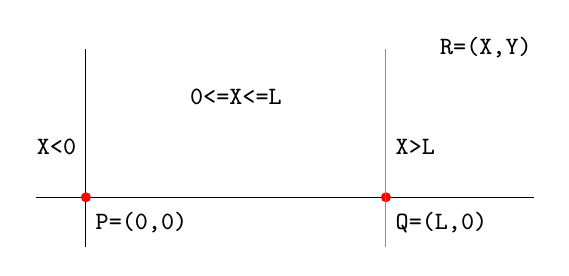
\begin{tikzpicture}[x=0.25in,y=0.25in]
\begin{scope}[>=triangle 45,shorten >=0.01in]

    \draw[black] (-1,0) -- (+9,0);
    \draw[black] (0,-1) -- (0,+3);
    \fill[red] (0,0) circle(0.1);
    \fill[red] (6.0,0) circle(0.1);
    \draw[brown] (6.0,-1) -- (6.0,+3);
    \draw[black] (0.0,-0.5) node[right]{\small \tt P=(0,0)};
    \draw[black] (6.0,-0.5) node[right]{\small \tt Q=(L,0)};
    \draw[black] (0.0,+1.0) node[left]{\small \tt X<0};
    \draw[black] (+6.0,+1.0) node[right]{\small \tt X>L};
    \draw[black] (+3.0,+2.0) node{\small \tt 0<=X<=L};
    \draw[black] (+8.0,+3.0) node{\small \tt R=(X,Y)};

\end{scope}
\end{tikzpicture}
\end{wrapfigure}
If we want the distance from {\tt r} to the \underline{finite} line {\tt pq},
then this is the same as {\tt 1/||q-p||} times
the distance from {\tt R} to the finite
line {\tt PQ}, and there are three cases.
If {\tt X<0}, the answer
is {\small \tt ||R-P||/||q-p||}.  If {\tt X>L},
the answer is {\small \tt ||R-Q||/||q-p||}.
Otherwise the answer is {\small \tt |Y|/||q-p||} as before.
See picture.
\end{minipage}

\medskip

Here we can simplify the above by using: \\
\begin{tabular}{@{~~}l}
\tt ||R-P||/||q-p|| = ||(q-p):(r-p)||/||q-p|| = ||r-p|| \\
\tt ||R-Q||/||q-p|| = ||(q-p):(r-q)||/||q-p|| = ||r-q|| \\
\end{tabular}

Now suppose we want a precise answer to the question: is {\tt r}
on the infinite or finite line {\tt pq}?  This is the same as the question:
is {\tt R} on the infinite or finite line {\tt PQ}?
If the coordinates of {\tt p}, {\tt q}, and {\tt r} have at
most {\tt d} decimal places, they are rational numbers with
denominator {\tt 10$^{\tt d}$}, and the products will be rational
numbers with denominator {\tt 10$^{\tt 2d}$}, so the coordinates of
{\tt R} and {\tt Q} will have denominator {\tt 10$^{\tt 2d}$}.
Or more precisely,
the computed coordinates will be close approximations to such rational numbers.
Therefore
\begin{enumerate}
\item {\tt r} is to the left of the infinite directed line {\tt pq}
if and only if {\tt 0<Y:(2d)}.
\item {\tt r} is to the right of the infinite directed line {\tt pq}
if and only if {\tt Y<0:(2d)}.
\item {\tt r} is on the infinite directed line {\tt pq}
if and only if {\tt Y==0:(2d)}.
\item {\tt r} is on the finite line {\tt pq} if and only if \\
\hspace*{0.3in}{\tt Y==0:(2d)},~~{\tt 0<=X:(2d)},~~and~~{\tt X<=L:(2d)}
\end{enumerate}

\newpage

\section{Line and Point Calculator}
Implement additions to the product calculator for
the following {\em operators} and {\em functions}:
\begin{center}
\begin{tabular}{l@{~~~~~}l@{~~~~~}l}
Assume: & {\tt p}, {\tt q}, {\tt r} are vectors representing points \\
	& {\tt d} is an integer scalar with {\tt 0 $\leq$ d $\leq$ 12} \\
then: \\[1ex]
\tt disti~pqr  & returns the distance from point {\tt r} to the
		\underline{infinite} line {\tt pq} \\
\tt distf~pqr  & returns the distance from point {\tt r} to the
		\underline{finite} line {\tt pq} \\
\tt closei~pqr  & returns the point {\tt t} on the \underline{infinite}
                  line {\tt pq} \\
		& that is closest to the point {\tt r} \\
\tt closef~pqr  & returns the point {\tt t} on the \underline{finite}
                  line {\tt pq} \\
		& that is closest to the point {\tt r} \\
\tt sidei~pqrd & returns {\tt +1} if {\tt r} is to the left of the
                \underline{infinite directed} line {\tt pq}, \\
	      & zero if it is on the line, and -1 if it is to the right, \\
	      & assuming all coordinates have at most {\tt d} decimal places \\
\tt onf~pqrd & returns {\tt true} if and only if {\tt r} is on the
                \underline{finite} line {\tt pq}, \\
	      & assuming all coordinates have at most {\tt d} decimal places \\
\end{tabular}
\end{center}

\begin{center}
\begin{tabular}{rl}
Sample Input Files: & \file{00-XXXX-point-vec-2d.in} \\
Sample Output Files: & \file{00-XXXX-point-vec-2d.ftest} \\
Sample Run File: & \file{sample-point-vec-2d.run} \\
Submit Run File: & \file{submit-point-vec-2d.run} \\
\end{tabular}
\end{center}

\newpage


\section{Line and Line}
In this section we investigate the following questions:
\begin{enumerate}
\item Do two infinite lines intersect, and if so where?
\item Do two finite lines intersect, and if so where?
\item What is the distance between two finite lines?
\end{enumerate}

Let {\tt p} and {\tt q} be a pair of distinct points so that the set
of points on the infinite line {\tt pq} is: \\
\centerline{{\tt K} = \{ {\tt p + s*(q-p)}: {\tt s} any scalar \}} 

Let {\tt m} and {\tt n} be another pair of distinct points so that the set
of points on the infinite line {\tt mn} is: \\
\centerline{{\tt K} = \{ {\tt m + t*(n-m)}: {\tt t} any scalar \}} 

If these two infinite lines intersect, there must exist values for
{\tt s} and {\tt t} such that: \\
\centerline{{\tt p + s*(q-p) = m + t*(n-m)}}

The easy way to solve this is to take the cross product of both
sides with {\tt n-m}, because
{\tt (n-m)\#(t*(n-m)) = t*((n-m)\#(n-m)) = t*0 = 0}.
So we end up with: \\
\centerline{\tt s*(n-m)\#(q-p) = (n-m)\#(m-p)} \\
which we can solve for {\tt s}.  Unless {\tt (n-m)\#(q-p) = 0}.

What happens if {\tt (n-m)\#(q-p) = 0}? \\
\hspace*{0.3in}\begin{tabular}{r@{~~}l}
Then    & \tt (n-m)\#(q-p) = sin $\theta$*||n-m||*||q-p|| = 0 \\
where   & \tt ||n-m|| $\neq$ 0 $\neq$ ||q-p|| \\
and     & \tt $\theta$ = azm (q-p) - azm (n-m) \\
so      & \tt sin $\theta$ = 0 \\
so      & \tt $\theta$ = 0 or $\pm$180 \\
so      & {\tt nm} and {\tt pq} are parallel \\
        \end{tabular}

The converse is also true.  If {\tt mn} and {\tt pq} are parallel, \\
\hspace*{0.3in}\begin{tabular}{r@{~~}l}
then    & {\tt azm (n-m) = azm (q-p)} \\
and     & \tt ||n-m|| $\neq$ 0 $\neq$ ||q-p|| \\
so      & {\tt n-m = s*(q-p)} for some scalar {\tt s} \\
so      & \tt (n-m)\#(q-p) = s*((q-p)\#(q-p)) = 0 \\
        \end{tabular}

Of course, testing a product to see if it is {\tt 0} is subject to
rounding errors.  So we assume that the coordinates of {\tt m},
{\tt n}, {\tt p}, and {\tt q} have at most {\tt d} decimal places,
and therefore {\tt mn} is parallel to {\tt pq} if and only if
{\tt (n-m)\#(q-p)==0:(2d)}.

If {\tt mn} and {\tt pq} are parallel infinite lines, they
may be disjoint or identical.  To test which, test whether
{\tt m} is on the infinite line {\tt pq} 

The question of whether two \underline{finite} lines intersect is made
simpler by the following:
\begin{lemma}
Two finite lines do \underline{not} intersect
if either does not intersect the infinite extension of the other.

Otherwise the two finite lines intersect at a single point unless
each finite line is a subset of the infinite extension of the other.
\end{lemma}
\begin{indpar}{0.3in}
Proof: The first statement is clear.

If one finite line is a subset of the the infinite extension of the
other, then the other finite line is a subset of the infinite extension
of the first finite line.

Otherwise let the finite lines be $\ell_1$ and $\ell_2$ and let
$\ell_i$ intersect the infinite extension of the other finite line
at single point $r_i$.  Then $r_1=r_2=$ the intersection of the infinite
extensions of both lines, and as $r_i$ is on $\ell_i$, this point is
on both finite lines.
\end{indpar}

If we have a finite line {\tt mn} and an infinite directed line extending
{\tt pq}, then we can test whether {\tt m} and {\tt n} are on, to the left of,
or to the right of the infinite directed line {\tt pq}, and we get the
following cases:
\begin{enumerate}
\item Both {\tt m} and {\tt n} are to the left of infinite {\tt pq}.
Then finite {\tt mn} does \underline{not} intersect infinite {\tt pq}.
\item Both {\tt m} and {\tt n} are to the right of infinite {\tt pq}.
Then finite {\tt mn} does \underline{not} intersect infinite {\tt pq}.
\item {\tt m} is to the left of and {\tt n} is to the right of infinite {\tt pq}.
Then finite {\tt mn} \underline{does} intersect infinite {\tt pq}.
\item {\tt m} is to the right of and {\tt n} is to the left of
infinite {\tt pq}.
Then finite {\tt mn} \underline{does} intersect infinite {\tt pq}.
\item Just one of {\tt m} or {\tt n} is on infinite {\tt pq}.
Then finite {\tt mn} \underline{does} intersect infinite {\tt pq}
at a single point.
\item Both {\tt m} and {\tt n} are on infinite {\tt pq}.
Then finite {\tt mn} is a \underline{subset} of the infinite {\tt pq}.
\end{enumerate}

The above cases can be captured by:
\begin{lemma}
If coordinates have at most {\tt d} decimal places,
a finite line {\tt mn} is a subset of an infinite line {\tt pq} if:
\\[1ex]
\centerline{{\tt (q-p)\#(m-p)==0:(2d)} and {\tt 0==(q-p)\#(n-p):(2d)}}

Otherwise the finite {\tt mn} intersects the infinite {\tt pq}
in a single point if:
\\[1ex]
\centerline{{\tt (q-p)\#(m-p)<=0:(2d)} and {\tt 0<=(q-p)\#(n-p):(2d)}} \\
\centerline{or} \\
\centerline{{\tt (q-p)\#(n-p)<=0:(2d)} and {\tt 0<=(q-p)\#(m-p):(2d)}}

Otherwise the finite {\tt mn} does \underline{not} intersect
the infinite {\tt pq}.
\end{lemma}

(Determining if {\tt mn} intersects or is a subset of infinite {\tt pq}
could be answered by evaluating \\
\centerline{{\tt ((q-p)\#(m-q))*((q-p)\#(n-q))<=0:(4d)}} \\
but the change from {\tt 2d} to {\tt 4d} is worrisome: {\tt 4d}
is often too large to be practical.)

If two finite lines intersect at a single point, the point of intersection
is the same as the point of intersection of the two infinite extensions
of the two finite lines, which we have determined at the beginning
of this section.

If the two infinite extensions of the two finite lines {\tt pq} and
{\tt mn} are the same
infinite line, we need a new approach.  We need to establish a coordinate
system on this infinite line.

If {\tt r} is a point on this infinite line then
{\tt r = p + s$_r$ * <q-p>} for some scalar {\tt s$_r$}.  Then
{\tt s$_r$ = $\pm$||r-p||} where the $+$ sign is chosen when {\tt r}
is to the same side of {\tt p} as {\tt q}, and the $-$ sign is chosen
when {\tt r} is to the opposite side of {\tt p} from {\tt q}.
We can use the map {\tt r $\mapsto$ s$_r$} as a system of coordinates
on the infinite line.

However it is more computationally convenient to use
{\tt r $\mapsto$ S$_r$ = (q-p)*r = ||q-p||*s$_r$} as the system of coordinates.
Distances in this coordinate system are {\tt ||q-p||} times distances in the
original coordinate system.

Using this coordinate system, the finite line {\tt pq} is represented
as the coordinate interval {\tt [S$_p$,S$_q$]}, where \\
\centerline{{\tt S$_p$ = (q-p)*(p-p) = 0} and {\tt S$_q$ = (q-p)*(q-p) > 0 }}
To simplify
the situation, switch {\tt m} and {\tt n} if necessary to that
{\tt S$_m$ < S$_n$} and {\tt mn} is represented by the coordinate
interval {\tt [S$_m$,S$_n$]}.  Then the overlap of the two intervals
is empty if {\tt S$_n$ < S$_p$} or {\tt S$_q$ < S$_m$}, and is
otherwise \\
\centerline{\tt [max(S$_p$,S$_m$),min(S$_q$,S$_n$)]}

We can summarize all this in:
\begin{lemma}
Given finite lines {\tt pq} and {\tt mn},
if coordinates have at most {\tt d} decimal places, if
\\[1ex]
\centerline{{\tt (q-p)\#(m-p)==0:(2d)} and {\tt 0==(q-p)\#(n-p):(2d)}}
\\[1ex]
(so each line is a subset of the infinite extension of the other line),
and if we switch {\tt m} and {\tt n} if necessary so that \\
\centerline{\tt (q-p)*(m-p) < (q-p)*(n-p)}
then
\begin{enumerate}
\item If {\tt (q-p)*(n-p) < (q-p)*(p-p):(2d)} the finite lines do not overlap.
\item If {\tt (q-p)*(q-p) < (q-p)*(m-p):(2d)} the finite lines do not overlap.
\item Otherwise the finite lines overlap and the length of the overlap \\
is {\tt (U-L {\rm rounded to} {\tt 2d} {\rm decimal places})/||q-p||} \\
\hspace*{0.5in}\begin{tabular}{rl}
where	& \tt L = max ( (q-p)*(m-p), (q-p)*(p-p) ) \\
and	& \tt U = min ( (q-p)*(n-p), (q-p)*(q-p) ) \\
\end{tabular} \\
(If we do not round {\tt U-L} it can happen that {\tt U-L < 0}.)
\end{enumerate}
\end{lemma}


Lastly we consider the problem of finding the distance between
the finite line {\tt mn} and the finite line {\tt pq}.  We assume:

\begin{theorem}
If {\tt mn} and {\tt pq} are finite lines, the function from pairs
of points
{\tt r$_{\tt mn}$} on {\tt mn} and
{\tt r$_{\tt pq}$} on {\tt pq}  to the distance
{\tt ||r$_{\tt mn}$ - r$_{\tt pq}$||} has a minimum.
\end{theorem}

We will \underline{not} give a proof of this,
which involves the mathematics of compact sets.

We will prove:

\begin{theorem}
\label{FINITE-LINE-DISTANCE-THEOREM}
If {\tt mn} and {\tt pq} are finite lines that do not intersect, then
points {\tt r$_{\tt mn}$} on {\tt mn} and
{\tt r$_{\tt pq}$} on {\tt pq} may be chosen so that
{\tt ||r$_{\tt mn}$ - r$_{\tt pq}$||} is minimal and
one of the chosen points is an end-point of its finite line.

Therefore the distance from {\tt mn} to {\tt pq} is the
smallest of: \\
\hspace*{0.5in}\begin{tabular}{l}
the distance from {\tt m} to {\tt pq} \\
the distance from {\tt n} to {\tt pq} \\
the distance from {\tt p} to {\tt mn} \\
the distance from {\tt q} to {\tt mn} \\
\end{tabular}
\end{theorem}

\begin{indpar}{0.3in}
Proof:  Consider the infinite line $\ell$ through
{\tt r$_{\tt mn}$} and {\tt r$_{\tt pq}$}, and assume that
neither
{\tt r$_{\tt mn}$} or {\tt r$_{\tt pq}$} are endpoints.
Then $\ell$ may be translated to its left or right by
a small enough amount that the translation continues
to intersect both finite lines.  Let the translation
be $\ell'$ and its intersections with the finite lines be
{\tt r'$_{\tt mn}$} and {\tt r'$_{\tt pq}$}.
If {\tt mn} and {\tt pq} are not parallel, then
{\tt ||r'$_{\tt mn}$ - r'$_{\tt pq}$||} will increase
as $\ell$ is translated in one direction and decrease as
it is translated in the other direction, but a decrease
cannot happen by assumption of minimality of
{\tt ||r$_{\tt mn}$ - r$_{\tt pq}$||}, so by contradiction either
{\tt r$_{\tt mn}$} or {\tt r$_{\tt pq}$} must be an endpoint.

If on the other hand {\tt mn} and {\tt pq} are parallel,
{\tt ||r'$_{\tt mn}$ - r'$_{\tt pq}$||} will remain constant
for all translations of $\ell$, and $\ell$ can be translated
in either direction until it encounters an endpoint.
\end{indpar}

The translation argument just given is an example of a
\key{perturbation argument}.  Perturbation arguments are common
in computational geometry.

Of course if the finite lines intersect the distance between
them is zero.

\newpage

\section{Line and Line Calculator}
Implement additions to the point and line calculator for
the following {\em operators} and {\em functions}:
\begin{center}
\begin{tabular}{l@{~~~~~}l}
Assume: & {\tt m}, {\tt n}, {\tt p}, {\tt q} are vectors representing points \\
	& {\tt d} is an integer scalar with {\tt 0 $\leq$ d $\leq$ 12} \\
then: \\[1ex]
\tt intersecti mnpqd & returns {\tt true} if the infinite lines {\tt mn} and
                     {\tt pq} \\
		   & intersect (including the case where the lines are \\
		   & identical) and {\tt false} otherwise; assuming point \\
		   & coordinates have at most {\tt d} decimal places \\
\tt intersectf mnpqd & ditto but for finite lines {\tt mn} and {\tt pq} \\
\tt overlapf mnpq & returns the length of the overlap of
                    finite lines {\tt mn} \\
                 & and {\tt pq} assuming the infinite extensions of these \\
		 & lines are identical \\
\tt commoni mnpq & returns the common point of infinite lines {\tt mn} and \\
                 & {\tt pq} assuming these lines are not parallel \\
\tt distf mnpq & returns the distance between finite lines {\tt mn} and
                  {\tt pq} \\
		& (may be zero if lines intersect) \\
\end{tabular}
\end{center}

\begin{center}
\begin{tabular}{rl}
Sample Input Files: & \file{00-XXXX-line-vec-2d.in} \\
Sample Output Files: & \file{00-XXXX-line-vec-2d.ftest} \\
Sample Run File: & \file{sample-line-vec-2d.run} \\
Submit Run File: & \file{submit-line-vec-2d.run} \\
\end{tabular}
\end{center}

\newpage


\section{Circle, Line, and Point}
In this section we investigate the following questions:
\begin{enumerate}
\item What is the distance between a point and a circle (viewed as
a curving line and \underline{not} an area)?
Is the point on the circle?
\item Where do the lines tangent to a circle that pass through
an external point contact the
circle?
\item Does an infinite line intersect a circle?  Is it
tangent to the circle?  Where does it intersect?
\item What is the distance between a finite line segment and
a circle?  If zero, where are the intersections?  If not zero,
where is the point on the finite line segment that is closest to the
circle.
\end{enumerate}

Suppose we have a point {\tt p} and a circle with center {\tt c}
and radius {\tt r>0}.  Then the distance from {\tt p} to the circle
is the absolute value of {\tt ||p-c|| - r},
where we view the circle as a closed line
and \underline{not} as an area.

To precisely test whether {\tt p} is outside, on, or inside the
circle, assuming that input coordinates and {\tt r} have at most
{\tt d} decimal places, we can use the equations:
\begin{center}
\begin{tabular}{l@{~~~~~}l}
\tt r$^2$ < (p-c)*(p-c):(2d) & outside the circle \\
\tt (p-c)*(p-c) == r$^2$:(2d) & on the circle \\
\tt (p-c)*(p-c) < r$^2$:(2d) & inside the circle \\
\end{tabular}
\end{center}


\begin{minipage}{\textwidth}\raggedright
\label{TANGENT-PICTURE}
\begin{wrapfigure}{r}{0.3\textwidth}
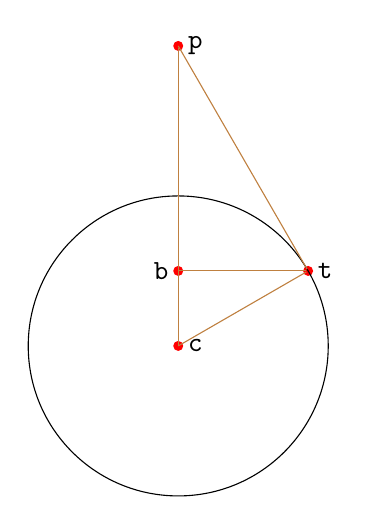
\begin{tikzpicture}[x=0.25in,y=0.25in]
\begin{scope}[>=triangle 45,shorten >=0.01in]

    \fill[red] (0,6.0) circle(0.1);
    \draw[black] (0,6.0) node[right]{\tt p};
    \fill[red] (0,0) circle(0.1);
    \draw[black] (0,0) node[right]{\tt c};
    \fill[red] (0,1.5) circle(0.1);
    \draw[black] (0,1.5) node[left]{\tt b};
    \fill[red] (2.598076,1.5) circle(0.1);
    \draw[black] (2.598076,1.5) node[right]{\tt t};


    \draw[black] (0,0) circle(3.0);
    \draw[brown] (0,0) -- (0,6.0);
    \draw[brown] (0,1.5) -- (2.598076,1.5);
    \draw[brown] (0,6.0) -- (2.598076,1.5);
    \draw[brown] (0,0) -- (2.598076,1.5);


\end{scope}
\end{tikzpicture}
\end{wrapfigure}
Now suppose that {\tt p} is outside the circle and we want to find
a point {\tt t} on the circle such that {\tt pt} is tangent to the
circle.  See the picture. \\
~ \\
\label{FINDING-TANGENT-POINT}
We define {\tt b} to be the point on {\tt pc} such that
{\tt tbp} is a right angle.  Then we have: \\
\hspace*{0.2in}\begin{tabular}{@{}l} \\
    {\tt ptc} is a right angle \\
    {\tt ||p-c||} is known \\
    {\tt ||t-c||=r} \\
    angle {\tt pct} equals angle {\tt tcb} \\
    triangles {\tt ptc} and {\tt tbc} are congruent \\
    so {\tt \small ||b-c||/||t-c|| = ||t-c||/||p-c||} \\
    so {\tt \small ||b-c|| = r$^2$/||p-c||} \\
    and using \\
    {\tt ||b-t|| = $\sqrt{{\tt r}^2 - {\tt ||b-c||}^2}$} \\
    we can compute both {\tt ||b-c||} and {\tt ||b-t||}; \\
    \end{tabular}
\end{minipage} \\
\hspace*{0.2in}\begin{tabular}{@{}l}
    then if we define {\tt u = <p-c>} we have \\
    {\tt b = c + ||b-c||*u = c + (r$^2$/L$^2$)*(p-c)} \\
    {\tt t \begin{tabular}[t]{@{}l}
         = b $\pm$ ||b-t||*(u\textasciicircum 90) \\
         = b $\pm$ (r/L$^2$)*$\sqrt{{\tt L}^2 - 1}$%
	                    *((p-c)\textasciicircum 90) \\
	   \end{tabular}} \\
    where {\tt L$^2$ = (p-c)*(p-c)} \\
    \end{tabular}

The reason for the $\pm$ is that we actually have two possible
values for {\tt t}, one on either side of the line {\tt pc}.

It turns out that the coordinates of {\tt b} are rational
with denominator containing {\tt (p-c)*(p-c)}.  However, the
coordinates of {\tt t} are irrational in general, due to
$\sqrt{\tt (p-c)*(p-c) - 1}$ being a factor while other factors are rational.
It comes down the the question of whether if {\tt p-c = 10$^{-d}$*(x,y)}
for integers {\tt x} and {\tt y}, then is
{\tt x$^2$+y$^2$-(10$^d$)$^2$} a perfect square.
For example, $101^2+201^2-100^2= 40602$ contains the factor $2$ only once
and is therefore not a perfect square.
Most of the time the sum will \underline{not}
be a perfect square, and so most of the time the
coordinates of {\tt t} will be irrational.

Now let {\tt p} and {\tt q} be points on an infinite line {\tt pq}
and let {\tt c} be a circle of radius {\tt r}.  Does {\tt pq} intersect
the circle, and is it tangent?

If {\tt pq} is tangent, the point {\tt t} where it intersects the
circle is also the point on the line closest to {\tt c}.  By
the argument on page \pageref{CLOSEST-IS-RATIONAL}, if
{\tt p}, {\tt q}, and {\tt c} all have rational coordinates, then
{\tt t} will have rational coordinates, but by the argument immediately
above, it will usually have irrational coordinates.  From this
we conclude that {\tt pq} is usually not tangent to the circle
if {\tt p}, {\tt q}, and {\tt c} all have rational coordinates and
{\tt r} is a rational number.

\bigskip

\begin{minipage}{\textwidth}\raggedright
\label{INTERSECTION-PICTURE}
\begin{wrapfigure}{r}{0.5\textwidth}
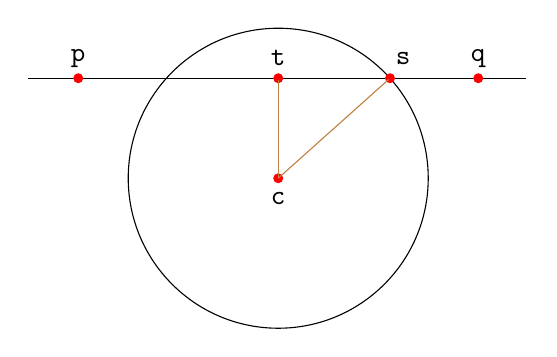
\begin{tikzpicture}[x=0.25in,y=0.25in]
\begin{scope}[>=triangle 45,shorten >=0.01in]

    \draw[black] (0,0) circle(3.0);
    \fill[red] (0,0.0) circle(0.1);
    \draw[black] (0,-0.4) node{\tt c};

    \draw[black] (-5.0,2.0) -- (+5.0,2.0);
    \fill[red] (-4.0,2.0) circle(0.1);
    \fill[red] (+4.0,2.0) circle(0.1);
    \draw[black] (-4.0,2.4) node{\tt p};
    \draw[black] (+4.0,2.4) node{\tt q};

    \fill[red] (0,2.0) circle(0.1);
    \draw[black] (0,2.4) node{\tt t};

    \draw[brown] (0,0) -- (0.0,2.0);

    \fill[red] (2.236068,2.0) circle(0.1);
    \draw[black] (2.5,2.4) node{\tt s};
    \draw[brown] (0,0) -- (2.236068,2.0);

\end{scope}
\end{tikzpicture}
\end{wrapfigure}
So let us just assume for the moment that the line intersects
the circle, and locate the points of intersection (see picture).
By section \ref{LINE-AND-POINT}, page \pageref{LINE-AND-POINT},
we can find the point {\tt t} on the line that is closest to
{\tt c}, and find the distance {\tt ||t-c||}.  Then the line {\tt tc} is
perpendicular to {\tt pq} as if it were not sliding {\tt t}
along the {\tt pq} line would reduce {\tt ||t-c||}.
If {\tt s} is an intersection point of {\tt pq} and the circle, we have: \\
\hspace*{0.2in}\begin{tabular}{@{}l}
    {\tt ||s-c||$^2$ = r$^2$ = ||t-c||$^2$ + ||t-s||$^2$} \\
    so {\tt ||t-s|| = $\sqrt{{\tt r}^2 - {\tt ||t-c||}^2}$} \\
    and if we define {\tt u = <q-p>} we have \\
    {\tt s = t $\pm$ ||t-s||*u} \\
    \end{tabular}
\end{minipage}

The reason for the $\pm$ is that we actually have two possible
values for {\tt s}, one on either side of the line {\tt tc}.

The distance {\tt ||t-s||} goes to zero as {\tt ||t-c||} approaches
{\tt r}, and cannot be computed if {\tt ||t-c|| > r}, in which case
the line is completely outside the circle and does not intersect the
circle.

We end this section by examining the case of a \underline{finite}
line {\tt pq} and a circle with center {\tt c} and radius {\tt r}.
Find the point {\tt t} on the infinite line {\tt pq} closest to
{\tt c}, and the points {\tt s} that where the infinite line intersects
the circle, if they exist.
Then use the {\tt (q-p)*} product to establish coordinates on the
infinite line: \\
\centerline{\tt (q-p)*p ~~~ (q-p)*q ~~~ (q-p)*t ~~~ (q-p)*s}
Since {\tt (q-p)*p~<~(q-p)*q},
{\tt t} is in the finite line {\tt pq} if and only if \\
\centerline{\tt (q-p)*p $\leq$ (q-p)*t $\leq$ (q-p)*q}
Similarly we can find out if an intersection point is on the finite
line.

So what points on the finite line {\tt pq} are closest to the circle?
If {\tt pq} intersects the circle these are the intersection points.
Otherwise there are two cases: {\tt pq} is outside the circle and
{\tt pq} is inside the circle.

To make further progress, we are \underline{not} going to use the fact that the
circle is a circle.
Instead we will use the fact that the circle viewed
as an area is a closed convex set, and the circle viewed as an arc
is the boundary of such a set.  This allows us to prove our results
for closed convex sets, and apply the results to circles, ellipses,
rectangles, and convex polygons.

\begin{definition}
The \key{boundary} of a set $S$ of the points in the plane
(i.e., $S\subset\mathcal{R}^2$) is the
set of points $p$ such that every circle with
center $p$ contains inside it a point in $S$ and another point not in $S$.

A set $S$ of points in the plane is \key{closed} if every point
of the boundary of $S$ is in $S$.

A set $S$ of points in a plane is a \key{bounded set} if and only if
there is a circle that includes $S$.
\end{definition}

We need $S$ to be closed in order to use the notion of
closest point.

\begin{lemma}\label{MINIMUM-DISTANCE}
Let $S_1$ and $S_2$ be close sets one of which is bounded.
Then there are points
$p_1\in S_1$ and $p_2\in S_2$ such that $||p_1-p_2||$ is as
small as possible (i.e., for every $q_1\in S_1$ and $q_2\in S_2$,
$||q_1-q_2||\ge||p_1-p_2||$).
\end{lemma}

We will \underline{not} give the proof of this,
which involves the mathematics of compact
sets (i.e., uses the fact that a closed bounded set is compact).

Some facts about boundaries are:
\begin{enumerate}
\item The boundary of a set $S$ is also the boundary of the
complement $\mathcal{R}^2-S$ of $S$.
\item The boundary $B$ of a set $S$ is itself closed
(i.e., $B$ is a closed set).
\end{enumerate}
\begin{indpar}{0.3in}
Proof:  The first fact is easy.  For the second fact, let
$p$ be a point in the
boundary of $B$.  Then every open circle centered at $p$
contains inside it a point $q$ in $B$ and a smaller circle
centered at $q$ that is inside the first circle, and this
smaller circule contains
inside it a point in $S$ and a point not in $S$.  So $p$ is in $B$.
\end{indpar}


Another important fact about closed sets and their boundaries is:

\begin{lemma}\label{BOUNDARY-CROSSING}
If $S$ is a closed set, $p$ is a point in $S$, and $q$ is a point
outside of $S$, then the finite line $pq$ contains a point on the
boundary of $S$.
\end{lemma}
\begin{indpar}{0.2in}
Proof: Consider the points $r=p+\alpha*(q-p)$ for $0\le\alpha\le 1$,
that is, the points $r$ on the finite line $pq$.
All circles with center $p$ contain a point of $S$ as $p$ is in $S$.
All sufficiently small circles with center $q$ contain only points
outside of $S$, as $q$ is outside of $S$ and not on the boundary of $S$
(which is a subset of $S$).  Let $\alpha'$ be the smallest number such
that $r=p+\alpha*(q-p)$ is outside $S$ for all $\alpha>\alpha'$ and
let $r_0=p+\alpha'*(q-p)$.  Then $r_0$ is in $S$, for if it were not,
a sufficiently small circle with center $r_0$ would be completely
outside $S$, and $\alpha'$ would be smaller than it is.  But every
circle with center $r_0$ includes a point $r=p+\alpha*(q-p)$,
$\alpha>\alpha'$ which
is outside of $S$.  So $r_0$ is on the boundary of $S$.
\end{indpar}

\begin{definition}
A set $S$ of the points in a plane
is a \key{convex set} if and only if for any two points $p$ and $q$ in $S$
and any scalar $0\le\alpha\le 1$,
$\alpha*p+(1-\alpha)*q \in S$
(i.e., the finite line segment $pq$ is in $S$).
\end{definition}

In order to deal with the case where the finite line $pq$ is
\underline{outside}
the circle, we will prove below:

\begin{theorem}\label{POINT-OUTSIDE-THEOREM}
The distance from a finite line $pq$ to a closed convex set $S$ when
$pq$ is \underline{outside} of $S$ is one of:
\begin{enumerate}
\item The distance from the infinite line $pq$ to $S$ if
a point on the infinite line closest to $S$ is in the finite line $pq$.
\item The distance from $p$ to $S$.
\item The distance from $q$ to $S$.
\end{enumerate}
\end{theorem}

Given this and a finite line {\tt pq} \underline{outside} the
circle,
we compute the point {\tt t} on the infinite line {\tt pq} that is
closest to the center of the circle
and check if that is in the finite line {\tt pq}.  If not, then the
closest point is either {\tt p} or {\tt q}, by the Theorem.

In order to deal with the case where the finite line $pq$ is
\underline{inside}
the circle, we will prove below:

\begin{theorem}\label{POINT-INSIDE-THEOREM}
The distance from a finite line $pq$ to the boundary of a
closed convex set $S$ when
$pq$ is \underline{inside} of $S$ is one of:
\begin{enumerate}
\item The distance from $p$ to the boundary of $S$.
\item The distance from $q$ to the boundary of $S$.
\end{enumerate}
\end{theorem}

The application of this theorem is obvious.

The rest of this secion just gives the proofs of the last two
theorems.

To prove Theorem~\ref{POINT-OUTSIDE-THEOREM}
we need a definition and some lemmas.

\begin{definition}
A function $F$ on a convex set of points $S$ is a \key{convex function}
if and only if
for any two points $p$ and $q$ in $S$ and
$0\le\alpha\le 1$,
$D(\alpha*p+(1-\alpha)*q)\le\alpha*F(p) + (1-\alpha)*F(q)$.
\end{definition}

Next note that for any two vectors $v_1$ and $v_2$,
\begin{center}
$|v_1*v_2|\le||v_1||*||v_2||$ \\
because $v_1*v_2 = ||v_1||*||v_2||*\cos\theta$ and $|\cos\theta|\le 1$ \\
where $\theta = \mathrm{azm}~v_2 - \mathrm{azm}~v_1$
\end{center}

Using this we prove:

\begin{lemma}
Let $S$ be a closed convex set and $pq$ be an infinite line.  For $r$ on $pq$,
define $D(r)$ to be the distance from $r$ to $S$ (distance of
$r$ to a point in $S$ closest to $r$).  Then $D(r)$ is a convex
function on the infinite line.
\end{lemma}
\begin{indpar}{0.2in}
Proof: \\
~\begin{tabular}[t]{l}
let $s_i$ be a point in $S$ closest to $r_i$ \\
let $r=\alpha*r_1+(1-\alpha)*r_2$
and $s=\alpha*s_1+(1-\alpha)*s_2$ \\
let $v_i=r_i-s_i$ and $v=r-s$ so $D(r_i)=||v_i||$ and $D(r)\le||v||$ \\
then \\
~$D(r)^2$\begin{tabular}[t]{@{}l}
    $\le v*v = (\alpha*v_1+(1-\alpha)*v_2)*(\alpha*v_1+(1-\alpha)*v_2)$ \\
    $= \alpha^2 v_1*v_1 + 2*\alpha*(1-\alpha)*v_1*v_2 + (1-\alpha)^2*v_2*v_2$ \\
    $\le \alpha^2*||v_1||^2 + 2*\alpha*(1-\alpha)*||v_1||*||v_2||
                           + (1-\alpha)^2*||v_2||^2$ \\
    $= (\alpha*||v_1|| + (1-\alpha)*||v_2||)^2$ \\
    $= (\alpha*D(r_1) + (1-\alpha)*D(r_2))^2$ \\
    \end{tabular} \\
so $D(r)\le\alpha*D(r_1)+(1-\alpha)*D(r_2)$
\end{tabular}
\end{indpar}

Note that if $r$ is in $S$, $D(r) = 0$.

\begin{lemma}
Let $F$ be a convex function on an infinite line,
let $p$ and $q$ be points on the line, and set $r=p+\alpha*(q-p)$
for some scalar $\alpha\ge 1$.  Then $F(r)\ge(1-\alpha)*F(p)+\alpha*F(q)$.
\end{lemma}
\begin{indpar}{0.2in}
Proof: $r-p = \alpha*(q-p)$ so $q-p=(1/\alpha)*(r-p)$ and as $F$ is convex,
$F(q)\le(1-1/\alpha)*F(p)+(1/\alpha)*F(r)$ from which the result
follows.
\end{indpar}

\begin{corollary}\label{CONVEX-EXTENSION}
If $F(q)> F(p)$ and $\alpha>1$ then $F(r)> F(p)$.
\end{corollary}

Now we have:

\begin{indpar}{0.2in}
Proof of Theorem \ref{POINT-OUTSIDE-THEOREM}:
By Lemma~\ref{MINIMUM-DISTANCE} there are points $r$ on the
finite line $pq$ that are closest to $S$.  If either $p$ or $q$ is
one of these points, we are done.  Otherwise
let $r_0$ be a point on the finite line $pq$ closest to $S$.
If $D(r)$ is the distance from $r$ to $S$ for $r$ on the infinite line $pq$,
we have $D(p)>D(r_0)<D(q)$ so from Corollary~\ref{CONVEX-EXTENSION}
$D(r)>D(r_0)$ for all $r$ on the infinite line $pq$ but outside the
finite line $pq$.  Therefore $r_0$ is a closest point to $S$ on the
infinite line $pq$.
\end{indpar}


To prove Theorem~\ref{POINT-INSIDE-THEOREM}
we need a definition and some lemmas.

\begin{definition}
For a set $S$ of points, the \key{convex hull} of $S$ is the
smallest convex set containing $S$.
\end{definition}

The convex hull is clearly the union of all finite lines {\tt pq} for
all pairs of points {\tt p} and {\tt q} in $S$.  The convex hull of
a convex set $S$ is clearly $S$ itself.
If $T$ is a subset of a convex set $S$,
the convex hull of $T$ is clearly a subset of $S$.

\begin{lemma}
Let $S$ be a closed convex set, let $p$ be a point in $S$, and
let $r$ be the distance from $p$ to the boundary of $S$.  Then
the circle of radius $r$ and center $p$ is completely within $S$.
\end{lemma}

\begin{indpar}{0.2in}
Proof:  By contradiction.  Assume there is a point $q$ on the circle
that is outside $S$.  Then by Lemma~\ref{BOUNDARY-CROSSING} there is
a point $s$ on the finite line segment $pq$ that is on the boundary of
$S$, and this cannot be $q$.  So $||s-p||<r$ which contradicts the
definition of $r$.
\end{indpar}

\begin{lemma}
Let $S$ be a closed convex set, let $p$ and $q$ be a points in $S$,
let $s=\alpha*p+(1-\alpha)*q$ for $0\le\alpha\le 1$ be a point on the
finite line $pq$, and let $r_p$, $r_q$, and $r_s$ be the distances
of $p$, $q$, and $s$ respectively from the boundary of $S$.
Then $r_s\ge\alpha*r_p+(1-\alpha)*r_q$.
\end{lemma}

\begin{indpar}{0.2in}
Proof:  By construction.  Let $r_s'=\alpha*r_p+(1-\alpha)*r_q$.
Let $C_p$ be the circle of center $p$ and
radius $r_p$, and let $C_q$ and $C_s'$ be constructed similarly from
$(q,r_q)$ and $(s,r_s')$.  Then we will prove $C_s'$ is a subset of
the convex hull of $C_p\cup C_q$, and as by the previous lemma
the latter is a subset of $S$, we get the conclusion $r_s\ge r_s'$.

Let $t$ be a point on the boundary $C_s'$ and let $v=t-s$, so
$||v||=r_s'$.  Let $v_p$ and $v_q$ be vectors
with the same direction (azimuth) as $v$ and lengths $r_p$ and $r_q$
respectively.  Then by hypothesis,
$||v|| = \alpha*||v_p||+(1-\alpha)*||v_q||$, so
$v = \alpha*v_p+(1-\alpha)*v_q$, and as
$s = \alpha*p+(1-\alpha)*q$, we have
$t=s+v=\alpha*(p+v_p)+(1-\alpha)*(q+v_q)$ and 
$t$ is on the finite line from $p+v_p$ to $q+v_q$ and is therefore in the
convex hull of $C_p\cup C_q$.
\end{indpar}



TBD


The points on the infinite line can be represented as
{\tt p+h*(q-p)} for scalars {\tt h}, and the square of the distance of such a
point from {\tt c} is then \\
\centerline{\tt (p+h*(q-p))*(p+h*(q-p))} \\
which is a quadratic
function of {\tt h}.  It has a minimum at {\tt p+h*(q-p) == t} and
is increasing as the point moves away from {\tt t}.

Therefore, if {\tt t} is on the finite line {\tt pq} it is the point on
that line closest to {\tt c}, and if {\tt t} is not on the line, either
{\tt p} or {\tt q} is the point closest to {\tt c}.  In either case
either {\tt p} or {\tt q} is the point farthest from {\tt c}.  Using
this information you can establish the minimum distance of the finite
line {\tt pq} from the circle viewed as a curved line (and \underline{not}
as an area).  You do not need to calculate intersection points {\tt s}
to determine whether there is an intersection.


\newpage

\section{Circle, Line, and Point Calculator}
Implement additions to the line and line calculator for
the following {\em operators} and {\em functions}:
\begin{center}
\begin{tabular}{l@{~~~~~}l}
Assume: & {\tt c}, {\tt p}, {\tt q} are vectors representing points \\
	& {\tt r} is a scalar with {\tt r > 0} \\
	& below the circle has center {\tt c} and radius {\tt r} \\
	& {\tt d} is an integer scalar with {\tt 0 $\leq$ d $\leq$ 12} \\
then: \\[1ex]
\tt sidec~crpd & returns {\tt -1} if {\tt p} is outside the circle, \\
               & {\tt 0} if it is on the circle, {\tt +1} if it is \\
	       & inside the circle, assuming all coordinates have \\
	       & at most {\tt d} decimal places \\
\tt distc crp  & returns the distance of the point {\tt p} to the  \\
               & circle viewed as an arc and not an area \\
\tt tangc crp  & returns a tangent point ({\tt t} in the page
                 \pageref{TANGENT-PICTURE} picture) \\
               & of a line through {\tt p} tangent to the circle; \\
	       & of the two possibilities, the one to the right of \\
	       & the directed line {\tt cp} must be returned \\
\tt basec crp  & returns the base point ({\tt b} in the page
                 \pageref{TANGENT-PICTURE} picture) \\
               & of lines through {\tt p} tangent to the circle; \\
	       & this is technically the point on {\tt cp} closest \\
	       & to the tangent point {\tt t} \\
\tt intersectc crpq  & returns the intersection point
                       ({\tt s} in the page \pageref{INTERSECTION-PICTURE} \\
               & picture) of the infinite line {\tt pq} and the circle; \\
	       & of the two possibilities, the one to the right of \\
	       & the directed line {\tt ct} must be returned, where \\
	       & {\tt t} is the point on the line closest to {\tt c} \\
\tt distc crpq  & returns the distance of the finite line {\tt pq} to the  \\
               & circle viewed as an arc and not an area \\
\end{tabular}
\end{center}

\begin{center}
\begin{tabular}{rl}
Sample Input Files: & \file{00-XXXX-circle-vec-2d.in} \\
Sample Output Files: & \file{00-XXXX-circle-vec-2d.ftest} \\
Sample Run File: & \file{sample-circle-vec-2d.run} \\
Submit Run File: & \file{submit-circle-vec-2d.run} \\
\end{tabular}
\end{center}

\newpage


\section{Ellipse, Line, and Point}
In this section we investigate the following questions:
\begin{enumerate}
\item How do you define an ellipse?
\item Where do the lines tangent to an ellipse that pass through
an external point contact the ellipse?
\item What is the distance between a point and an ellipse (viewed as
a curving line and \underline{not} an area)?
Is the point on the ellipse?
\item Does an infinite line intersect an ellipse?  Is it
tangent to the ellipse?  Where does it intersect?
\item What is the distance between a finite line segment and
a circle?  If zero, where are the intersections?  If not zero,
where is the point on the finite line segment that is closest to the
ellipse.
\end{enumerate}

A circle with center at {\tt (0,0)} and radius {\tt r} is the set:
\begin{center}
$\{ (x,y) : (\frac{x}{r})^2 + (\frac{y}{r})^2 = 1 \}
=
\{ (r\cos\theta,r\sin\theta): 0\leq\theta< 2\pi \}$
\end{center}

An \key{ellipse} with center at {\tt (0,0)}, \key{major axis} {\tt M}
and \key{minor axis} {\tt m}, with the major axis in the X-axis direction
(the minor axis is always perpendicular to the major axis) is the set:
\begin{center}
$\{ (x,y) : (\frac{x}{M})^2 + (\frac{y}{m})^2 = 1 \}
=
\{ (M\cos\theta,m\sin\theta): 0\leq\theta< 2\pi \}$
\end{center}


\begin{minipage}{\textwidth}\raggedright
\label{INTERSECTION-PICTURE}
\begin{wrapfigure}{r}{0.5\textwidth}
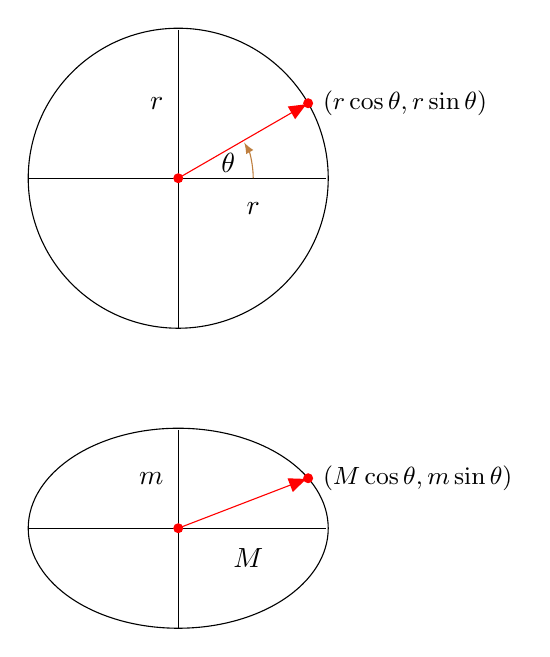
\begin{tikzpicture}[x=0.25in,y=0.25in]
\begin{scope}[>=triangle 45,shorten >=0.01in]

    \draw[black] (-3.0,0) -- (3.0,0);
    \draw[black] (0,-3.0) -- (0,3.0);
    \fill[red] (0,0.0) circle(0.1);
    \draw[black] (-0.1,1.5) node[left]{$r$};
    \draw[black] (1.5,-0.6) node{$r$};

    \draw[black] (0,0) circle(3.0);
    \fill[red] (2.598076,1.5) circle(0.1);
    \draw[red,->] (0,0) -- (2.598076,1.5);
    \draw[black] (2.7,1.5) node[right]{\small$(r\cos\theta,r\sin\theta)$};

    \draw[brown,>=latex,->] (1.5,0) arc(0:30:1.5);
    \draw[black] (1.0,+0.3) node{$\theta$};

    \draw[black] (-3.0,-7.0) -- (3.0,-7.0);
    \draw[black] (0,-9.0) -- (0,-5.0);
    \fill[red] (0,-7.0) circle(0.1);
    \draw[black] (0,-7.0) ellipse(3.0 and 2.0);
    \draw[black] (-0.1,-6.0) node[left]{$m$};
    \draw[black] (1.4,-7.6) node{$M$};

    \fill[red] (2.598076,-6.0) circle(0.1);
    \draw[red,->] (0,-7.0) -- (2.598076,-6.0);
    \draw[black] (2.7,-6.0) node[right]{\small$(M\cos\theta,m\sin\theta)$};

\end{scope}
\end{tikzpicture}
\end{wrapfigure}
Lets call a circle with center {\tt (0,0)} a \key{reference circle}.
Then an arbitrary circle is made by translating the reference circle
so its center is moved to an arbitrary point. \\
~ \\
Lets call an ellipse with center {\tt (0,0)} and major axis aligned with
the X-axis a \key{reference ellipse}.
Then an arbitrary ellipse is made by first rotating the reference ellipse
to align its major axis in an arbitrary direction, and then
translating it so its center is moved to an arbitrary point. \\
~ \\
Conversly, if you have an arbitrary ellipse, a translation followed
by a rotation will turn it into a reference ellipse.  So we are only
going to consider reference ellipses in this section.
\end{minipage}

\medskip

The reference circle with unit radius is closely related to
the reference ellipse by the linear transformation: \\
\centerline{$L = (M*u_x,m*u_y): (x,y) \longmapsto (M*x,m*y)$} \\
This is because: \\
\centerline{$L*(\cos\theta,\sin\theta) = (M*\cos\theta,m*\sin\theta)$}

More explicitly, let $S$ be any set of points in ${\mathcal R}^2$
and define $L * S = \{ L*p: p \in S \}$.
Let $C$ be the reference circle of radius 1, which we will
call the \key{reference unit circle}, and let $E$ be the reference
ellipse with major axis $M$ and minor axis $m$.

Then $L*C = E$.

This is important because of the following.

First, note that $L^{-1}$, the inverse of $L$, exists (where we assume
$M,m>0$) and is such that \\
\centerline{$L^{-1} = (M^{-1}*u_x,m^{-1}*u_y): (x,y)
            \longmapsto (M^{-1}*x,m^{-1}*y)$} \\
\centerline{$L^{-1}*(M*\cos\theta,m*\sin\theta) = (\cos\theta,\sin\theta)$} \\
so $L^{-1}*E=C$.

Then
\begin{itemize}
\item If $S$ is a straight line tangent to $C$, then $L*S$ is a straight
line tangent to $E$.
\item If $S$ is a straight line tangent to $E$, then $L^{-1}*S$ is a straight
line tangent to $C$.
\end{itemize}

In general, for any linear transformation $\mathcal{L}$ and straight line
$S$, $\mathcal{L}*S$ is a straight line.  This is because for some point
$p$ and vector $v$, \\
\hspace*{0.5in}\begin{tabular}{ll}
$S$ & $= \{ p+s*v : s~\mathrm{is~a~scalar}\}$ \\
$\mathcal{L}*S$
    & $= \{ \mathcal{L}*(p+s*v) : s~\mathrm{is~a~scalar}\}$ \\
    & $= \{ \mathcal{L}*p+s*(\mathcal{L}*v) : s~\mathrm{is~a~scalar}\}$ \\
\end{tabular} \\
That is, linear transformations `preserve' straight lines.

Also, if $\mathcal{L}$ is a 1-1 map (as both $L$ and $L^{-1}$ are),
and if $S_1$ and $S_2$ are two sets of points, then
$\mathcal{L}*(S_1\cap S_2) = (\mathcal{L}*S_1)\cap(\mathcal{L}*S_2)$.
That is, intersections are `preserved'.  A straight line is tangent
to an ellipse or circle if and only if the two intersect in a single
point, and as intersections and straight lines are preserved, tangency
is preserved by $L$ and $L^{-1}$.

Now consider the problem of finding the point $t$ on the reference ellipse
where a straight line passing through a point $p$ external to the
ellipse and tangent to the ellipse touches the ellipse.  Then
$T=L^{-1}*t$ is the point on $C$ where a straight line passing through
the point $P=L^{-1}*p$ and tangent to $C$ touches $C$.  Using the
methods of page~\pageref{FINDING-TANGENT-POINT} we can find $T$ and
therefore $t=L*T$.

Now consider the problem of finding the point $q$ on the reference ellipse
that is closest to $p$.  Let $t_1$ and $t_2$ be the two points on the
reference ellipse where straight lines passing through $p$ and tangent
to the ellipse touch the ellipse.  Let $P=L^{-1}*p$, $Q=L^{-1}*1$,
$T_1=L^{-1}*t_1$, $T_2=L^{-1}*t_2$.
Let $\theta=\mathrm{azm}~Q$,
$\theta_1=\mathrm{azm}~T_1$,
$\theta_2=\mathrm{azm}~T_2$.
We know $\theta_1$ and $\theta_2$ and want to find $\theta$.
See picture.

The key fact is that the tangent to the ellipse at $q$ must be perpendicular
to the line $pq$.  If it were not, sliding $q$ along the ellipse in one
direction would decrease $||q-p||$.  Let the direction of the line tangent
to the ellipse at \\
\centerline{$q_\phi = (M*\cos\phi,m*\sin\phi)$} \\
be given by a vector $v_\phi$.
Then the function $F(\phi)=<q_\phi-p>*<v_\phi>$ is $0$ at $\phi=\theta$
and monotonic between $\phi=\theta_1$ and $\phi=\theta_2$.  If we can compute
$F(\phi)$ from $\phi$, we can use binary search to compute $\theta$.

As $q_\phi = (M*\cos\phi,m*\sin\phi)$ the problem reduces to computing $v_\phi$.
Let $Q_\phi = L^{-1}*q_\phi = (\cos\phi,\sin\phi)$ and
$V_\phi=L^{-1}*v_\phi$.  Then this last is the direction of the tangent
to $C$ at $Q_\phi$, and we can take this direction as
$R^{90}*Q=(-\sin\phi,\cos\phi)$ so we can take
$V_\phi=(-\sin\phi,\cos\phi)$ and therefore $v_\phi=(-M*\sin\phi,m*\cos\phi)$.
Now doing the binary search finds $\theta$.



\bigskip

\begin{tabular}{ll}
Author:	      & Robert L.~Walton $<$walton@acm.org$>$ \\
Date:         & Wed Jan  6 18:44:00 EST 2021

\end{tabular}

The authors have placed this problem in the public domain;
they make no warranty and accept no liability for this problem.

\end{document}
